%============ standard packages ===============%
\documentclass[11pt]{report}\usepackage[utf8]{inputenc}
\usepackage[nottoc,numbib]{tocbibind}
\usepackage[parfill]{parskip}
\usepackage{mathtools}
\usepackage{hyperref}
\usepackage{natbib}
\bibliographystyle{agsm}
\usepackage{amsmath}
\usepackage{mathabx}
\usepackage{xcolor}
%============ packages for algorithms ===============%
\usepackage{algorithm,algorithmic}
%============ packages for spacing ===============%
\usepackage[a4paper,
    left=1.3in,
    right=1in]{geometry}
\usepackage{setspace}
\renewcommand{\baselinestretch}{1.4}
\setcounter{tocdepth}{2}
\usepackage{scrextend}
\usepackage{lscape}
\usepackage{fancybox}
\usepackage{etoolbox}
\patchcmd{\abstract}{\null\vfil}{}{}{}
%============ packages for figures ===============%
\usepackage{graphicx}
\usepackage{subcaption}
%============ packages for tables ===============%
\usepackage{booktabs}
\usepackage{array}
%============ commands for theorems etc ===============%
\newtheorem{assump}{A}
\renewcommand\theassump{(\arabic{assump})}
\newtheorem{bound}{B}
\renewcommand\thebound{(\arabic{bound})}
\newtheorem{condition}{C}
\renewcommand\thecondition{(\arabic{condition})}
\newtheorem{theorem}{Theorem}

\newcommand\independent{\protect\mathpalette{\protect\independenT}{\perp}}
\def\independenT#1#2{\mathrel{\rlap{$#1#2$}\mkern2mu{#1#2}}}

\begin{document}
%============ title page ===============%

\begin{titlepage}
\begin{center}
\rule[0.5ex]{\linewidth}{2pt}\vspace*{-\baselineskip}\vspace*{3.2pt}
\rule[0.5ex]{\linewidth}{1pt}\\[\baselineskip]
{\HUGE \Large Screening High Dimensional Time Series via Tilting}\\[0.5cm]
\rule[0.5ex]{\linewidth}{1pt}\vspace*{-\baselineskip}\vspace{3.2pt}
\rule[0.5ex]{\linewidth}{2pt}\\[2.5cm]


\includegraphics[width = 0.9\textwidth]{../plots/LSE_logo.png}\\[2.5cm]

\textbf{Department of Statistics 2019}\\[0.5cm]
\textit{A thesis submitted for the degree of Master of Science}\\
\textit{London School of Economics, University of London}\\[0.5cm]
\textit{Candidate: 13185}\\
\textit{Supervisor: Professor Piotr Fryzlewicz}
\end{center}
\end{titlepage}

%\cleardoublepage
\renewcommand\thepage{\romannumeral\numexpr\value{page}\relax}

\begin{abstract}
Developing effective feature screening procedures when the number of features exceeds the sample size $(p \gg n)$ is one of the most active research areas in modern statistics. Although much attention has been devoted to the problem of detecting causal and predictive relationships in high dimensional regimes, comparatively little attention has been given to the problem of developing general purpose screening procedures for high dimensional time series data. This is especially surprising given high dimensional time series are becoming increasingly common in many fields including economics, finance, and neuro-science. 

The aim of this dissertation is to adapt tilted correlation screening, a variable selection procedure for linear models introduced by \cite{cho2012high}, to settings in which the response, predictor, and error variables are allowed to be time series processes. Overall, the dissertation aims to make the following original contributions: 
\begin{enumerate}
    \item Show that under mild assumptions the main theoretical results in \cite{cho2012high} hold for time series data. 
    \item Introduce a generalised least squares variant of the tilted correlation which is more efficient than the original (in the Gauss-Markov / MSE sense). 
    \item Apply the principle of stability selection introduced by \cite{meinshausen2010stability} to tilted correlations when the correlation structure of the predictor variables necessitates careful control.
\end{enumerate}

The theoretical results presented are reinforced by simulation studies. Additionally, a real data application is provided in which tilted correlation screening is used to select a model for forecasting CPI inflation, chained GDP, and the Sterling effective exchange rate.

\bigskip
\bigskip

\textbf{Key words:} high dimensionality, mixing, sparsity, tilting, time series, variable screening.
\end{abstract}

\renewcommand{\abstractname}{Acknowledgements}
\begin{abstract}
I would like to extend my deepest gratitude to my supervisor, Professor Piotr Fryzlewicz, firstly for agreeing to supervise this project and secondly for giving up so much of his time to guide me through the research process. I would also like to thank Professor Clifford Lam who first interviewed me for the ESRC Studentship which has funded my masters. Finally I would like to thank Dr Yining Chen for introducing me to parallel computing, without which this dissertation would have take roughly seven times longer to write. 
\end{abstract}

\setcounter{tocdepth}{1}
\tableofcontents
\listoffigures
\listoftables

\cleardoublepage
\pagenumbering{arabic}
\chapter{Introduction} \label{introduction}

The need to analyse vast quantities of data is becoming increasingly common across most-all disciplines. By way of example, 90 percent of the world's data in 2013 had been generated in the last two years - see \cite{Bigdata}. Motivated by the growing challenges posed by `Big Data', this dissertation studies the broad problem of selecting features for a high dimensional linear model with the additional requirement that the data may be from a time series process. The main contribution is the extension of tilted correlation screening (TCS), a variable selection procedure for linear models introduced by \cite{cho2012high}, to the time series setting. 

High dimensionality refers to the setting in which the number of features present in a dataset exceeds the number of observations $(p \gg n)$. At the most fundamental level high dimensionality rules out parameter estimation by least squares (the workhorse of modern statistics), as the number of equations to be solved will by construction be smaller than the number of unknowns. Moreover, spurious collinearity among predictors and noise accumulation have been shown to degrade the properties of feature screening procedures which perform well in traditional settings; see \cite{fan2010selective} for an overview. The most popular approach to model building in high dimensions has been to invoke the sparsity assumption: a prior belief that only a subset of features $(s \ll n)$ is relevant to the relationship of interest. The assumption has lead to two methodologies. These are penalised estimation methods such as the Lasso of \cite{tibshirani1996regression} and its many variants, and screening methods such as Sure Independence Screening of \cite{fan2008sure} and its variants.

While existing methodologies have been widely adopted, most assume i.i.d. observations and are therefore poorly suited to the time series setting. High dimensional time series are nonetheless common in many fields. Examples can be found in neuro-science - see for example \cite{valdes2005estimating}, macroeconomics - see \cite{stock2002macroeconomic}, and finance - see \cite{choi2019high}. Moreover, even when the original dataset is not highly dimensional, uncertainty over the functional form with which each feature enters into the model often leads practitioners to take transformations of features (polynomials, splines, interactions, etc.) which can result in a very large number of `technical' features, see for example \cite{belloni2014inference}. The need to advance the literature on general purpose screening procedures is therefore clear. 

The dissertation is structured as follows. The remainder of Chapter \ref{introduction} briefly reviews the existing literature on general purpose screening procedures for high dimensional time series, and introduces notation used throughout the dissertation. Chapter \ref{techniques} formally introduces the TCS algorithm of \cite{cho2012high}, and presents popular techniques from the high dimensional literature which will be used to extend tilted correlations to the time series setting. Original contributions are presented in Chapter \ref{extensions}: Section \ref{seperation} investigates the properties of tilted correlations in a time series setting, while in Sections \ref{efficient tilting} and \ref{stable tilting} propose two extensions which exploit the time series setting to improve the screening accuracy of the original procedure. Chapter \ref{numerical} investigates the screening properties of tilted correlations in high dimensional time series through simulation studies and a real data example. Chapter \ref{conclusion} offers some concluding remarks. Finally, note that R code for simulation studies and data analysis carried out in this dissertation in available via \href{https://github.com/Shakeel95/ST499-Tilting-}{GitHub}. 

\section{Approach to screening high dimensional time series}

\cite{fan2008sure} spearheaded feature screening screening for high dimensional linear models with Sure Independence Screening (SIS). The procedure functions by ranking each feature according to its marginal utility. Specifically, let $\boldsymbol{\omega} = \left ( \omega_1,...,\omega_p \right )^T=\boldsymbol{X}^TY$ be a vector of coefficients obtained vai $p$ component-wise regressions where the response $Y$ and each column of the design matrix $\boldsymbol{X}$ have been standardised and de-meaned. Defining $d_n$ to be a stopping index which may grow with the sample size, for example $d_n = \text{floor}\left \{ n/\log n \right \}$, the subset of features selected by SIS is obtained via: 

\begin{equation*}
    \widehat{\mathcal{M}} = \left \{ 1 \leq j \leq p : \left | \omega_j \right | \text{ is among the } d_n\right \text{ largest}\}
\end{equation*}

Under reasonably mild assumptions the authors show that with probability approaching one the true set of relevant features $\mathcal{M}_*$ is contained within the chosen subset: $\mathbb{P}\left ( \mathcal{M}_* \subset \widehat{\mathcal{M}} \right ) \rightarrow 1$ as $n \rightarrow \infty$. Fan \& Lv coin this the `sure screening property'. Although SIS as proposed by \cite{fan2008sure} assumes i.i.d. observations, subsequent papers have worked to relax the assumption. In particular, a handful of recent papers propose SIS-like procedures adapted to the time series setting. 

\cite{yousuf2018variable} first showed that SIS continues to exhibit the sure screening property in a time series setting. Specifically the paper assumes a linear model where random variables are required to be strictly stationary and ergodic time series, and dependence between ordered observations is quantified via the functional dependence measure proposed in \cite{wu2005nonlinear}. Extending TCS to the time series setting is nonetheless worthwhile, as for reasons explored in Section \ref{tilting introduction} TCS tends to outperform SIS. To better account for the correlation structure of time series data, the paper introduces an efficient extension to SIS in which marginal utilities are estimated via generalised least squares (GLSS). In this dissertation the same extension is applied to tilted correlations in Section \ref{efficient tilting}. 

Motivated by the observation that when forecasting real time series nonlinear models can often outperform linear models, see for example \cite{terasvirta2010modelling}, two recent extensions to SIS focus on screening nonlinear time series. \cite{yousuf2018partial} proposes model free screening methods based on ranking distance and partial distance co-variance measures introduced by \cite{szekely2007measuring} and \cite{szekely2014partial} respectively. The assumptions are similar to those in \cite{yousuf2018variable}, and both methods have the sure screening property. Meanwhile \cite{chen2018semiparametric} suggest a kernel based variant of SIS (KSIS), which assigns marginal utilities by performing p component-wise kernel regressions; the rationale being that kernel regressions are consistent for any specification of the conditional mean as long as the target function is sufficiently smooth. 

\section{Model setup and notation} \label{setup}

The dissertation considers the setting where $\left \{ y_t \right \}_{t=1}^{n}$ represents a collection of scalar observations from a stationary time series process; $d_n$ lags are potentially relevant, and additionally there are $q_n$ exogenous predictors $z_{tj}$. In total there are $p_n = q_n + d_n$ potential predictors and the set of predictors is denoted by $\mathcal{J} = \left \{ 1, ..., p_n \right \}$. Both $d_n$ and $q_n$ may diverge as the sample size increases. The predictors are expressed as follows:

\begin{equation*} \label{predictors}
    x_{tj} = \left\{\begin{matrix}
    z_{tj} \hspace{1cm} j = 1,...,q_n\\ 
    y_{t-(j-q_n)} \hspace{1cm} j = q_n+1,...,q_n+d_n
\end{matrix}\right.
\end{equation*}

The relationship between the predictor and response variables is assumed to be linear, and is given by $Y = \mathbb{X} \boldsymbol{\beta} + \boldsymbol{\epsilon}$ where $\boldsymbol{\epsilon}$ is an $n \times 1$ vector of errors. To cope with potential high dimansionality the linear relationship is assumed to be sparse in the sense that $\mathcal{S} = \left \{ j \in \mathcal{J} : \beta_j \neq 0 \right \}$ with $\left | \mathcal{S} \right | = s < n $. 

For notational convenience $\mathbf{X}$ denotes an $n \times p_n$ matrix where the j-th column is an $n \times 1$ vector of observations for the j-th predictor re-scaled according to $x_{tj}^\text{scaled} = \frac{x_{tj} - \overline{x}_j}{\widehat{\sigma}_j}$, with $\overline{x}_j = n^{-1}\sum_t x_{tj}$ and $\widehat{\sigma}_j = \sqrt{n^{-1} \sum_t\left ( x_{tj} - \overline{x}_j \right )^2}$; entries in $Y$ are scaled accordingly. Such re-scaling is not typically applied to time series as it fundamentally alters the dependence structure of the data - in a sense each observation now contains the whole sample. The re-scaling is only used for variable screening, and the difficulties introduced by re-scaling are dealt with explicitly in Section \ref{seperation}. This being said, note that standardised and de-meaned time series have been directly used for forecasting by, among others, \cite{song2011large} and \cite{de2008forecasting}, who simply re-attribute mean and variance to the forecast. 

The j-th column of $\mathbf{X}$ is an $n \times 1$ vector denoted by $X_j$. The sub-matrix of $\mathbf{X}$ whose columns are predictors in the set $\mathcal{D}$ is expressed as $\mathbf{X}_\mathcal{D}$. A $p \times 1$ vector of predictors observed at time $t$ and not re-scaled is expressed as $\boldsymbol{x}_t$. Finally, $\mathring{\mathbf{Z}}$ denotes a matrix scaled by $\frac{1}{\sqrt{n}}$. The sample correlation matrix can therefore be written as $\mathbf{C} = \mathring{\mathbf{X}}^T\mathring{\mathbf{X}} = \left ( c_{j,k} \right )_{j,k = 1}^{p_n}$. 

\chapter{Techniques} \label{techniques}

\section{Tilted correlation screening}\label{tilting introduction}

The tilted correlation of \cite{cho2012high} is a measure of association designed to remedy two pitfalls of marginal correlation screening algorithms identified by \cite{fan2008sure}, specifically: 

\begin{enumerate}
    \item Irrelevant variables which are highly correlated with relevant ones can have high priority to be selected in marginal correlation screening. 
    \item A relevant variable can be marginally uncorrelated but jointly correlated with the response.
\end{enumerate}

The following decomposition of the marginal correlation between an arbitrary predictor $X_j$ and the response shows that these pitfalls can be attributed to a `bias term' which depends on predictors in the set $\mathcal{S} \setminus \left \{ j \right \}$: 

\begin{equation*}
    \mathring{X}_j^T\mathring{Y} = \mathring{X}_j^T\left ( \sum_{k=1}^{p_n} \beta_k \mathring{X}_k + \mathring{\boldsymbol{\epsilon}}  \right ) = \beta_j + \underbrace{\sum_{k \in \mathcal{S} \setminus \left \{ j \right \}} \beta_k \mathring{X}_j^T\mathring{X}_k}_\text{bias} + \mathring{X}_j^T\mathring{\boldsymbol{\epsilon}} 
\end{equation*}

For completeness I note that Fan \& Lv address these pitfalls through Iterative Sure Independence Screening (ISIS): a procedure which repeatedly applies SIS to residuals obtained by regression the response variable on predictors selected by SIS. This however is computationally expensive. 

\subsubsection{The tilting procedure}

Tilted correlations work by transforming each predictor so that the associated bias term is negligible or zero. Since knowledge of the set $\mathcal{S}$ is impossible, the authors note that the bias contribution is largest for those predictors which attain a large sample correlation with $X_j$. For each predictor, a set of highly correlated predictors is constructed as $\mathcal{C}_{j} = \left \{ k \neq j : \left | \mathring{X}_j^T \mathring{X}_k \right | > \pi_{n}  \right \}$, where $\pi_n$ effectively acts as a hard threshold on the sample correlation matrix. A de-biased or tilted predictor can then be constructed by projecting onto the space orthogonal to the space spanned by members of the set $\mathcal{C}_j$. 

\begin{figure}[h]
    \centering
    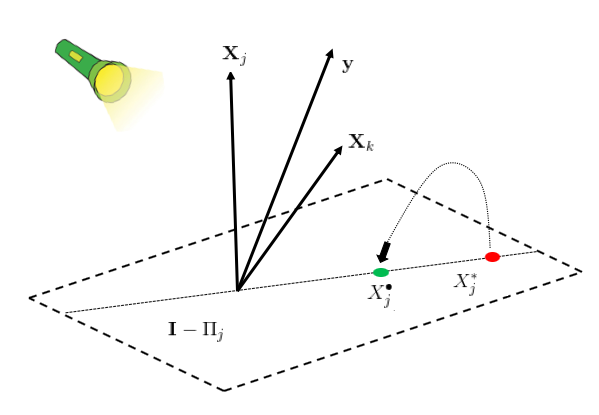
\includegraphics[width = 0.5\linewidth]{../plots/Tilting intuition.png}
        \caption{The tilting procedure visualised in $\mathbb{R}^3$. With $\mathcal{C}_j = \left \{ k \right \}$, $X_j$ is projected onto the orthogonal compliment of the space spanned by $X_k$ and re-scaled.}
    \label{graphical tilt}
\end{figure}

Defining the projection matrix $\Pi_j \equiv \boldsymbol{X}_{\mathcal{C}_j} \left ( \boldsymbol{X}_{\mathcal{C}_j}^T \boldsymbol{X}_{\mathcal{C}_j} \right )^{-1}\boldsymbol{X}_{\mathcal{C}_j}^T$, the tilted counterpart of each j-th predictor is $X_j^* \equiv  \left ( \boldsymbol{I}_n - \Pi_j \right )X_j$. Provided the set $\mathcal{C}_j$ is non-empty it holds that $\left \| \mathring{X}_j^* \right \|_2^2 = \mathring{X}_j^T\left ( \boldsymbol{I}_n - \Pi_j \right ) \mathring{X}_j < \mathring{X}_j^T\mathring{X}_j = 1 $, hence $\left ( \mathring{X}_j^* \right )^T \mathring{Y}$ cannot be used directly as a measure of association. To address this the authors propose two re-scaling methods. The first, on which this dissertation shall focus, is motivated by the decomposition below: 

\begin{align*}
    \left ( \mathring{X}_j^* \right )^T\mathring{Y} & = \mathring{X}_j^T \left ( \boldsymbol{I}_n -\Pi_j \right )\left \{ \sum_{k=1}^{p_n} \beta_k \mathring{X} + \mathring{\boldsymbol{\epsilon}} \right \} \\
    & = \beta_j\mathring{X}_j^T\left ( \boldsymbol{I}_n - \Pi_j \right )\mathring{X}_j + \sum_{k \in \mathcal{S} \setminus \mathcal{C}_j,k\neq j}\beta_k\mathring{X}_j^T\left ( \boldsymbol{I}_n - \Pi_j \right )\mathring{X}_k + \mathring{X}_j^T\left ( \boldsymbol{I}_n - \Pi_j \right )\mathring{\boldsymbol{\epsilon}}
\end{align*}

Provided the second and third terms are small, re-scaling by $\mathring{X}_j^T (\boldsymbol{I}_n-\Pi_j) \mathring{X}_j$ isolates $\beta_j$, which amounts to isolating the contribution of the j-th predictor to the response. The j-th tilted correlation is therefore defined as: 

\begin{equation*}
    c_j^* = \left ( \mathring{X}_j^* \right )^T\mathring{Y} / \left ( \mathring{X}_j^T (\boldsymbol{I}_n-\Pi_j) \mathring{X}_j \right )
\end{equation*}

Figure \ref{graphical tilt} gives a graphical representation of the tilting procedure. Note that when $\mathcal{C}_j = \emptyset$ the tilted correlation between a predictor and the response collapses to the marginal correlation. In this way, tilted correlations make an adaptive choice between the traditional Pearson's (straight) correlation and a measure which corrects for the linear contribution of other highly correlated predictors. 

\subsubsection{Threshold selection procedure}

A careful choice of the set $\mathcal{C}_j$ is crucial in high dimensional settings. We would like the set to including all predictors which contribute to the bias term, however if the membership of $\mathcal{C}_j$ is too large when $p \gg n$ any vector in $\mathbb{R}^n$ can be closely approximated by a linear combination of predictors in the set; the tilted correlation will therefore fail to capture any relationship between a given predictor and the response. The parameter $\pi_n$ determines membership of $\mathcal{C}_j$. 

Cho \& Fryzlewicz propose selecting $\pi_n$ by performing a hypothesis test of the form $H_0:\left | \Sigma_{j,k} \right | = 0 $ on each off-diagonal entry of $\boldsymbol{C}$, the sample correlation matrix of $\boldsymbol{X}$. Their procedure is set out in Algorithm \ref{threshold algorithm} below, and is an adaptation of the procedure in \cite{el2008spectrum} which controls the expected false discovery rate at a pre-set level $v^*$. This dissertation follows the original paper in setting $v^* = p^{-\frac{1}{2}}$. 

\begin{algorithm} 
\caption{Threshold selection procedure}
\begin{algorithmic}[1] \label{threshold algorithm}
  \scriptsize
  \STATE Set $n \leftarrow \text{nrow}(\boldsymbol{X})$; $p \leftarrow \text{ncol}(\boldsymbol{X})$; $d \leftarrow p(p-1)/2$
  \STATE Generate an $n \times p$ matrix $\boldsymbol{W}$, where each entry is distributed according to $\mathcal{N}(0,1)$
  \STATE Obtain reference sample correlations from $\boldsymbol{W}$ of the form $\left \{ r_{l,m} : 1\leq l< m \leq p \right \}$
  \STATE Assign p-values for each hypothesis test as $P_{j,k} \leftarrow d^{-1}\left | \left \{ r_{l,m} : 1 \leq l < m \leq p, \left | r_{l,m} \right | \geq \left | c_{j,k} \right | \right \} \right |$
  \STATE Sort p-values in ascending order $P_{(1)} \leq ... \leq P_{(d)}$
  \STATE Choose the largest $i$ such that $P_{(i)} \leq i / d \cdot v^*$
  \STATE Set $\pi_n$ to be the absolute value of the sample correlation corresponding to $P_{(i)}$
\end{algorithmic}
\end{algorithm}

\subsubsection{The separation property}

The main theoretical result in \cite{cho2012high} is the `separation property', which states that under appropriate conditions tilted correlations can separate between relevant and irrelevant predictors. More formally $\mathbb{P}\left ( \Delta  \right )\rightarrow 0$ where the event $\Delta$ is defined as: 

\begin{equation*}
    \Delta = \left \{  \frac{|c_k^*|}{\min_{j \in \mathcal{S}}|c_j^*|} \rightarrow 0 \textit{  for all  } k \notin \mathcal{S} \right \}
\end{equation*}

The authors employ the six assumptions listed below when studying the theoretical properties of tilted correlations. In what follows a deterministic sequence $\left \{ a_n \right \}_{n=1}^\infty$ is said to be $\mathcal{O}(b_n)$, where $\left \{ b_n \right \}_{n=1}^\infty$ is another deterministic sequence, if $\lim_{n \rightarrow \infty} \left | \frac{a_n}{b_n} \right | = c $ for some positive constant $c$.  

\begin{assump} \label{A1}
    The number of non-zero coefficients satisfies $\left | \mathcal{S} \right | = \mathcal{O}\left ( n^\delta \right )$ for $\delta \in \left [ 0,1/2 \right )$.
\end{assump}

\begin{assump} \label{A2}
    The number of predictors satisfies $\log\left ( p_n \right ) = \mathcal{O}\left ( n^\theta \right )$ for $\theta \in [0,1-2\gamma) $ with  $\gamma \in  \left ( \delta, 1/2 \right )$. 
\end{assump}

\begin{assump} \label{A3}
The threshold for membership of each set $\mathcal{C}_j$ satisfies $\pi_{n} = \mathcal{O}\left ( n^{-\gamma} \right )$, and the cardinality of each $\mathcal{C}_j$ satisfies $\left | \mathcal{C}_j \right | = \mathcal{O}\left ( n^{\xi } \right )$ for $ \xi \in \left [  0, 2\left ( \gamma - \delta  \right ) \right ) $.
\end{assump} 

\begin{assump} \label{A4}
    The largest non-zero coefficient satisfies $\max_{1 \leq j \leq p_n} \left | \beta_j \right | < M $ for $M \in \left ( 0, \infty \right )$.
\end{assump}

\begin{assump} \label{A5}
    For each $j \in \mathcal{J}$ it holds that $1 - \mathring{X}_j^T\Pi_j\mathring{X}_j = 1 - a_j >  a $ for $a \in \left ( 0,1 \right )$.
\end{assump}

\begin{assump} \label{A6}
    For those $j$ whose $\mathcal{C}_j$ satisfies $\mathcal{S} \nsubseteq \mathcal{C}_j$, for some $\kappa$ satisfying $\kappa/2 + \mu \in [0, \gamma - \delta - \xi/2)$ it holds that $n^\kappa \cdot \frac{\left \| \left ( \boldsymbol{I}_n-\Pi_j \right )\boldsymbol{X}_\mathcal{S}\boldsymbol{\beta}_\mathcal{S} \right \|_2^2}{\left \| \boldsymbol{X}_\mathcal{S}\boldsymbol{\beta}_\mathcal{S} \right \|_2^2} \rightarrow \infty$
\end{assump}

A\ref{A1} and A\ref{A2} describe how the sparsity $|\mathcal{S}|$ and dimensionality $p_n$ of the linear model may grow with the sample size $n$. A\ref{A3} requires that the number of predictors in each $\mathcal{C}_j$ does not exceed a certain polynomial rate in $n$, which is needed in order to guarantee the existence of each projection matrix $\Pi_j$. Finally, A\ref{A5} rules out strong collinearity among predictors, which agan guarantees the existance of each projection matrix. For a full discussion of the assumptions see \textit{Section 2.3} of the original paper. 

\subsubsection{Tilted correlation screening algorithm}

Algorithm \ref{tilting algorithm} below sets out the TCS algorithm  as described in \textit{Section 3.1} of the original paper. The algorithm exploits the theoretical properties of tilted correlations, and selects a set of predictors of size $m<n$ which contains the true set $\mathcal{S}$ with high probability. The algorithm generates a solution path $\mathcal{A}_{(1)} \subset ... \subset \mathcal{A}_{(m)}$, hence the final model $\widehat{\mathcal{S}}$ is obtained either by selecting a model from the solution path or by selecting a subset of predictors from the final active set. 

\bigskip

\begin{algorithm} 
\caption{Tilted Correlation Screening}
\begin{algorithmic}[1] \label{tilting algorithm}
  \scriptsize
  \STATE Begin with an empty active set $\mathcal{A} = \emptyset$, current residual equal to the response variable $W=Y$, and current design matrix $\boldsymbol{Z = X}$. From $\boldsymbol{X}$ obtain a correlation threshold $\pi_n$. 
  \STATE Find the variable which achieves the maximal marginal correlation with $W$, and let $k = \arg \max_{j \notin \mathcal{A}}\left | Z_j^TW \right |$. Identify the set of $\mathcal{C}_k = \left \{ j \notin \mathcal{A}, j \neq k : \left | Z_j^TZ_k \right | > \pi_n \right \}$. If $\mathcal{C}_j = \emptyset$ set $k^* = k$ and go to Step 4. 
  \STATE If $\mathcal{C}_k \neq \emptyset$ screen the tilted correlation $c_j^*$ between $Z_j$ and $W$ for each $j \in \left \{ \left \{ k \right \} \cup \mathcal{C}_k \right \}$. Set $k^* = {\arg-\max}_{j \in \left \{ \left \{ k \right \} \cup \mathcal{C}_k \right \}} \left | c_j^* \right |$. 
  \STATE Add $k^*$ to the active set $\mathcal{A} \leftarrow \mathcal{A} \cup\left \{ k^* \right \}$, and update the current residual $W \leftarrow \left ( \boldsymbol{I}_n-\Pi_\mathcal{A} \right )Y$ and current design matrix $\boldsymbol{Z} \leftarrow \left ( \boldsymbol{I}_n-\Pi_\mathcal{A} \right )\boldsymbol{X}$. Re-scale each column $j \notin \mathcal{A}$ to have $l_2$-norm 1. 
  \STATE Repeat Steps 2-4 until the cardinality of the active set reaches $\left | \mathcal{A} \right |$ a pre-specified value $m<n$. 
\end{algorithmic}
\end{algorithm}

\section{Measures of Dependence}\label{measures of dependence}

Beginning around the time of \cite{rosenblatt1956central} statisticians realised the usefulness of measure of dependence for time series that do not fit any specific dependence structure but have some asymptotic notion of independence. To make the results in this dissertation as general as possible the same approach is used. Mixing conditions are one such class of measure which capture the idea that dependence between observations should decay as they get further apart. 

\subsection{Strong Mixing}

Throughout the dissertation $\alpha$-mixing (henceforth strong mixing) is used, however for completeness I introduce four of the most common mixing conditions. Let $\left \{ Z_t, t \in \mathbb{Z} \right \}$ be an ordered sequence of random variables equipped with a probability triple $\left ( \Omega, \mathcal{F}_{-\infty}^\infty, \mathbb{P} \right )$, the common mixing conditions are the following: 

\begin{align*} \label{mixing condition}
    & \alpha(n) := \sup_{j \in \mathbb{Z}} \left \{ \sup_{\mathcal{A} \in \mathcal{F}_{- \infty}^j,\mathacal{B} \in \mathcal{F}_{j+n}^\infty} \left | \mathbb{P}\left ( \mathcal{A} \cap \mathcal{B}\right ) - \mathbb{P}\left ( \mathcal{A}\right )\mathbb{P}\left (  \mathcal{B}\right ) \right |  \right \} \\
    & \beta(n) = \sup_{\mathcal{A},\mathacal{B}} \frac{1}{2} \sum_{i=1}^{I} \sum_{j=1}^{J} \left | \mathbb{P}\left ( \mathcal{A}_i \cap \mathcal{B}_j\right ) - \mathbb{P}\left ( \mathcal{A}_i\right )\mathbb{P}\left ( \mathcal{B}_j \right ) \right | \nonumber \\
    & \phi(n) := \sup_{j \in \mathbb{Z}} \left \{ \sup_{\mathcal{A} \in \mathcal{F}_{- \infty}^j,\mathacal{B} \in \mathcal{F}_{j+n}^\infty} \left | \mathbb{P}\left ( \mathcal{B} | \mathcal{A} \right ) - \mathbb{P}\left (  \mathcal{B}\right )\right | \right \} \nonumber \\
    & \psi(n) := \sup_{j \in \mathbb{Z}} \left \{  \sup_{\mathcal{A} \in \mathcal{F}_{- \infty}^j,\mathacal{B} \in \mathcal{F}_{j+n}^\infty} \left | \frac{\mathbb{P}\left ( \mathcal{A} \cap \mathcal{B}\right )}{\mathbb{P}\left ( \mathcal{A}\right )\mathbb{P}\left (  \mathcal{B}\right )} - 1 \right | \right \} \nonumber
\end{align*}

If $\alpha(n) \rightarrow 0$ as $n \rightarrow \infty$ the process generating $\left \{ Z_t, t \in \mathbb{Z} \right \}$ is said to be strong mixing. Clearly when $\left \{ Z_t, t \in \mathbb{Z} \right \}$ is a sequence of $\text{i.i.d.}$ random variables all four measures are exactly zero for any $n>0$ - $\text{i.i.d.}$ random variables are simply a special case of mixing sequences. Indeed, as long as the mixing coefficient decays to zero sufficiently fast many properties of $\text{i.i.d.}$ processes, in particular laws of large numbers and central limit theorems, can be established for mixing processes. For a detailed survey of mixing conditions and their properties see \cite{bradley2005basic}. The following inequality is well known:

\begin{equation*}
    2\alpha(n) \leq \beta(n) \leq \phi(n) \leq \frac{1}{2}\psi(n)
\end{equation*}.

Strong mixing was chosen because it is implied by the other mixing conditions, and is therefore the easiest to satisfy. Indeed, a large class of commonly studied time series processes have been shown to be strong mixing. For example ergodic Markov chains are strong mixing, stationary ARMA processes are geometrically strong mixing - see \cite{mokkadem1988mixing}, and even ARCH($\infty$) processes have been shown to be strong mixing with mixing coefficient depending on the rate of decay of the ARCH parameters - see \cite{fryzlewicz2011mixing}.  

\subsection{Inequalities for strong mixing processes} \label{exponential inequalities}

Here I present some inequalities for strong mixing processes from \cite{bosq2012nonparametric} which will be of use throughout Chapter \ref{extensions}. In what follows $\left \{ Z_t, t \in \mathbb{Z} \right \}$ is a zero mean strong mixing process with $S_n = Z_1 + ... +Z_n$ being a partial sum, and $X$ and $Y$ are real valued random variables. 

\begin{bound} \label{B1}
    Rio's inequality. Let $Q_X(u) = \inf \left \{ t : \mathbb{P}\left ( \left | X \right | > t \right ) \leq u \right \}$ be the quantile function for $\left | X \right |$ and define $\alpha = \alpha \left ( \sigma (X), \sigma (Y) \right )$, if $Q_XQ_Y$ is integrable over $(0,1)$ it holds that: 
\begin{equation*}
    \left | \text{Cov}\left ( X,Y \right )  \right | \leq  2\int_{0}^{2 \alpha} Q_X(u)Q_Y(u)du
\end{equation*}    
    
\end{bound}

\begin{bound} \label{B2}
    If $\left \{ Z_t, t \in \mathbb{Z} \right \}$ is bounded, i.e. $\mathbb{P}\left ( \sup_t \left | Z_t \right | \leq b \right ) = 1$ for some $b \in (0, \infty)$, for each integer $q \in \left [ 1,\frac{n}{2} \right ]$ and for any $\epsilon > 0$ it holds that:
\end{bound} 

\begin{equation*}
    \mathbb{P}\left ( \left | S_n \right | > n \epsilon \right ) \leq 4 \exp\left ( -\frac{\epsilon^2}{8b^2} q \right ) + 22\left ( 1+\frac{4b}{\epsilon} \right )^{\frac{1}{2}}q\alpha\left ( \left [ \frac{n}{2q} \right ] \right )
\end{equation*}

\begin{bound} \label{B3}
    If the process satisfies the Cramér condition, i.e. there exists some constant $c>0$ such that for all $t \in \mathbb{R}$ and for integer each $k \geq 3$ it holds that $\mathbb{E}\left | Z_t \right |^k\leq c^{k-2} k! \mathbb{E}\left ( Z_t^2 \right )$, with the same $q$ and $\epsilon$ as B\ref{B2} it holds that: 
\end{bound}

\begin{equation*}
    \mathbb{P}\left ( \left | S_n \right | > n \epsilon \right ) \leq a_1 \exp\left ( -\frac{q\epsilon^2}{25m_2^2+5c\epsilon} \right )+a_2(k)\alpha\left ( \left [ \frac{n}{q+1} \right ] \right )^\frac{2k}{2k+1}
\end{equation*}

\textit{where $a_1$ and $a_2(k)$ are defined as follows:} 

\begin{equation*}
    a_1 = 2\frac{n}{q}+2\left ( 1+\frac{\epsilon^2}{25m_2^2 + 5c \epsilon} \right ) \hspace{0.5cm} \textit{with} \hspace{0.2cm} m_2^2 = \max_{1\leq t\leq n} \mathbb{E}(Z^2_t)
\end{equation*}

\begin{equation*}
    a_2(k) = 11n\left ( 1 + \frac{5m_k^{\frac{k}{2k+1}}}{\epsilon} \right ) \hspace{0.5cm} \textit{with} \hspace{0.2cm} m_k = \max_{1\leq t\leq n} \left \| Z_t \right \|_k
\end{equation*}

Exponential concentration inequalities such as B\ref{B2} and B\ref{B3} have become a mainstay of the high dimensional literature as they allow statisticians to derive bounds which tighten with $n$ without explicitly accounting for the behaviour of $p_n$; see for example chapter 2 of \cite{wainwright2019high}. In particular \cite{chen2018semiparametric} use B\ref{B3} to prove that KSIS has the sure screening property. 


\section{Bootstrapping}

The bootstrap of \cite{efron1992bootstrap} is a widely used re-sampling technique which generates pseudo-samples $\boldsymbol{Z}^* = \left \{ Z_{1}^*,...,Z_{n}^* \right \}$ from an observed sample $\boldsymbol{Z} = \left \{ Z_{1},...,Z_{n} \right \}$ by sampling with replacement from the empirical distribution. Recent papers, for example \cite{meinshausen2010stability} and \cite{christinelse}, have successfully applied re-sampling to the problem of estimating `stable' models for high dimensional data by performing variable selection on the basis of inclusion frequencies. In this section I briefly review extensions of the bootstrap whose pseudo-samples retain salient features of the original sample, and are therefore well suited to the high dimensional time series setting. These ideas will be useful in Section \ref{stable tilting}. 

\subsection{Bootstrapping stationary time series} \label{Bootstrapping ts}

Time series are characterised by a natural temporal ordering, as well as some structured dependence between observations. Efron's bootstrap is therefore poorly suited to the time series setting, as sampling randomly from the empirical distribution will destroy the dependence structure of the original sample. \cite{kunsch1989jackknife} suggest breaking the original sample into $k$ blocks of size $b_n$, i.e. $\boldsymbol{Z} = \left \{ \boldsymbol{B}_{1,b_n},...,\boldsymbol{B}_{n-b_n+1,b_n} \right \}$, and instead sampling blocks of observations. Each block is defined as:  $\boldsymbol{B}_{i,b_n} = \left \{ Z_i, Z_{i+1},...,Z_{i+b_n-1} \right \}$

If $b_n$ is chosen so that $ n = k b_n$ for some integer $k$ with $b_n \rightarrow \infty$ and $b_n/n \rightarrow 0$ as $n \rightarrow \infty$ then each block can be treated as approximately independent from every other block. Importantly, since within each block observations are grouped according to their natural order the `block bootstrap' preserves the dependence structure of the original sample. 

If $\boldsymbol{Z}$ is a sample from a strictly stationary time series then by construction $\boldsymbol{Z}^* = \left \{ \boldsymbol{B}_1^*,..., \boldsymbol{B}_k^*\right \}$ will be non-stationary. This is because the pseudo-sample will contain a structural break every $b_n$ observations. To remedy this, \cite{politis1994stationary} propose the `stationary bootstrap'. Let $\left \{ L_1, L_2,... \right \}$ be $\text{i.i.d.}$ with geometric distribution such that $\mathbb{P}\left ( L_1 = t \right ) = r\left ( 1-r \right )^{t-1}$ for some positive integer $r$, and let $\left \{ I_1, I_2,... \right \}$ be $\text{i.i.d.}$ with discrete uniform distribution on $\left \{ 1,...,n \right \}$. A `stationary bootstrap' sample is generated by setting  $\boldsymbol{Z}^{*} =\left \{ \boldsymbol{B}_{I_1,L_1},\boldsymbol{B}_{I_2,L_2},... \right \}$ until the desired length is reached. The dependence structure in the original sample is preserved by the same reasoning as in the `block bootstrap'. Additionally, structural breaks are now random so $\boldsymbol{Z}^{*}$ will be strictly stationary given $\boldsymbol{Z}$.  

For completeness I note that there exist a large number of parametric bootstrap schemes for time series data; for a concise overview see \textit{Chapter 9} of \cite{shao2012jackknife}. These however assume that the form of the model generating $\boldsymbol{Z}$ is known explicitly. By the desire for generality expressed in Section \ref{measures of dependence} such methods are not explored. 

\subsection{Bootstrapping high dimensional data}

As the limit of $p_n/n$ grows $\boldsymbol{Z}^*$'s ability to faithfully replicate meaningful features of $\boldsymbol{Z}$ deteriorates. This is clearest from the fact that the empirical distribution of the bootstrap weights, i.e. the number of times any given $Z_t$ is included in the bootstrap sample, has  asymptotic $\text{Poisson}(1)$ distribution; for a proof see \textit{Proposition 4.10} in \cite{el2010high}. A direct consequence is that the expected number of unique $Z_t$s in any bootstrap sample is $n\left ( 1-\frac{1}{\exp(1)} \right ) \approx 0.63 n$. As observed by \cite{karoui2016can}, if $p_n/n \gg 0.63$ then each $\boldsymbol{Z}^*$ will be asymptotically rank deficient even if $\boldsymbol{Z}$ has full column rank. This problem is clearly exacerbated by the `block bootstrap' and its variants. 

\chapter{Extensions} \label{extensions}
\section{Proving the separation property}\label{seperation}

The first step in applying the TCS algorithm to time series data is to show that the separation property continues to hold in the time series setting. In \cite{cho2012high} the separation property is proven by observing that the sample correlation between the response $y_t$ any predictor $x_{tj}$ projected onto the space orthogonal to the space spanned by predictors in $\mathcal{C}_j$ can be decomposed as follows:

\begin{align} \label{bounding}
    (\mathring{X}_j^*)^T\mathring{Y} & = \mathring{X}_j^T(\mathbf{I}-\Pi_j)\mathring{Y} \nonumber \\
    & = \mathring{X}_j^T \left \{ \sum_{k=1}^{p} \beta_k (\mathbf{I} - \Pi_j)\mathring{X}_k + (\mathbf{I} - \Pi_j)\mathring{\boldsymbol{\epsilon}}  \right \} \nonumber \\ 
    & = \beta_j \mathring{X}_j^T(\mathbf{I} -
     \Pi_j)\mathring{X}_j + \underbrace{\sum_{k \in \mathcal{S} \setminus  \mathcal{C}_j, k \neq j } \beta_k \mathring{X}_j^T (\mathbf{I} - \Pi_j) \mathring{X}_k}_{1} + \underbrace{\mathring{X}_j^T(\mathbf{I} - \Pi_j) \mathring{\boldsymbol{\epsilon}}}_{2} 
\end{align}

Terms 1 and 2 are shown to be negligibly small, and after appropriate re-scaling the remaining term does not depend on the sample size and is exactly zero for irrelevant predictors. The original proof relies on a well known concentration inequality for Gaussian random variables. I present a similar proof which instead uses the exponential inequalities introduced in Section \ref{exponential inequalities} and is therefore valid for a large class of time series processes. The proof uses assumptions A\ref{A1}-A\ref{A6} from the original paper, however to adapt to the time series setting three additional assumptions are required. 

\subsubsection{Additional assumptions}

\begin{assump} \label{A7}
    The process $\left \{ \left ( y_t, \boldsymbol{x}_t, \epsilon_t \right ), t \in \mathbb{Z} \right \}$ is a strictly stationary $\alpha$-mixing process with mixing coefficient having size $\alpha(n) = \mathcal{O}(\alpha^n)$ for $\alpha \in (0,1)$.
\end{assump}

\begin{assump} \label{A8}
    For all $t \in \mathbf{Z}$ and all $j \in \mathcal{J}$ it holds that $x_{tj} \independent \epsilon_t$.
\end{assump}

\begin{assump} \label{A9}
    Letting $Z_t = x_{tj} \cdot \epsilon_t$ for any $j \in \mathcal{J}$ it holds that $\mathbb{E}Z_t = 0$ for all $t$ and either: (i) $Z_t$ is bounded as in B\ref{B2}, or (ii) $Z_t$ satisfies the Cramér condition as in B\ref{B3}.
\end{assump}

A\ref{A7} is a standard assumption in the econometric literature: it allows us to quantify the degree of dependence in the data while being agnostic towards the data generating process itself. Specifically, A\ref{A7} restricts the degree of dependence to that of a geometrically strong mixing process. The same assumption is made in all of the screening methods presented in \cite{chen2018semiparametric}. A\ref{A8} imposes independence between the model errors and each predictor, and allows us to split the expectation of a product into the product of expectations when using the Markov inequality in the proofs below; it may be seen as somewhat restrictive, as in general it is sufficient to assume that the errors and predictors are contemporaneously uncorrelated. In the high dimensional setting however it is not unreasonable to assume that the set of predictors is sufficiently rich to justify complete independence. Finally, A\ref{A9} is necessary in order to make use of the exponential inequalities introduced in Section \ref{exponential inequalities}. In the unbounded case it implies all moments of the errors and predictors are finite. 


\subsection{A proof for scenario 1} \label{scenario 1}

\textit{Scenario 1} in the original paper refers to the setting in which whenever $X_j$ is projected onto the space spanned by predictors in the associated set $\mathcal{C}_j$ any relevant predictors not in $\mathcal{C}_j$ remain remain `far away' from the projection. The setting is expressed formally as: 

\begin{condition}\label{C1}
    $\left | \left ( \Pi_j \mathring{X}_j \right )^T \mathring{X}_k \right | = \mathcal{O}\left ( n^{-\gamma} \right )$ for all $j \in \mathcal{J}$ and $k \in \mathcal{S} \setminus \left \{ \mathcal{C}_j \cup \left \{ j \right \} \right \}$. 
\end{condition}

In a time series setting, whenever C\ref{C1} holds the tilted correlations of relevant predictors dominate those of irrelevant predictors.

\bigskip

\fbox{
\begin{minipage}{\columnwidth}
    \begin{theorem} \label{theorem 1}
    Under assumptions A\ref{A1}-A\ref{A9} and the additional condition C\ref{C1} it holds that $\mathbb{P}(\Delta)\rightarrow 1$, where the event $\Delta$ is defined as: 
    
    \begin{equation*}
        \Delta = \left \{  \frac{|c_k^*|}{\min_{j \in \mathcal{S}}|c_j^*|} \rightarrow 0 \textit{  for all  } k \notin \mathcal{S} \right \}
    \end{equation*}
    \end{theorem}
\end{minipage}
}

\bigskip

\textbf{Proof:}

For those $j$ whose $\mathcal{C}_j$ satisfy $\mathcal{S} \setminus \left \{ j \right \} \subseteq \mathcal{C}_j$ it follows that $\mathcal{S} \setminus \left \{ \mathcal{C}_j \cup \left \{ j \right \}  \right \} = \emptyset$ and term 1 will be exactly zero. When $\mathcal{S} \setminus \left \{ j \right \} \nsubseteq \mathcal{C}_j$ term 1 typically will not be zero, however we can bound: 

\begin{equation*}
    \left | \mathring{X}_j \left ( \mathbf{I} - \Pi_j\right ) \mathring{X}_k \right | \leq \left | \mathring{X}_j^T \mathring{X}_k \right | + \left | \left ( \Pi_j \mathring{X}_j \right )^T \mathring{X}_k \right | \leq Cn^{-\gamma}
\end{equation*}

Where the second inequality comes from the fact that A\ref{A3} guarantees that for each $k \notin \mathcal{C}_j$ $\left | \mathring{X}_j^T \mathring{X}_k \right |$ will be smaller that $\pi_{n}$, which in turn is bounded from above by $Cn^{-\gamma}$. Hence, term 1 can be bounded as follows: 

\begin{equation*}
    \left | \sum_{k \in \mathcal{C} \setminus  \mathcal{C}_j, k \neq j } \beta_k \mathring{X}_j^T (\mathbf{I} - \Pi_j) \mathring{X}_k \right | \leq  C\left | \mathcal{S} \right |n^{-\gamma} \leq Cn^{-(\gamma-\delta)}
\end{equation*}

Which holds because A\ref{A1} guarantees that $\left | \mathcal{S} \right | \leq Cn^{\delta}$ and A\ref{A4} guarantees that the largest $|\beta_j|$ is bounded away from infinity. It remains to show that with probability approaching one term 2 does not exceed the upper bound established for term 1. Since $\mathring{X}_j^T \mathring{\boldsymbol{\epsilon}}$ is proportional to $\mathring{X}_j^T \Pi_j\mathring{\boldsymbol{\epsilon}}$ by assumptions A\ref{A3} and A\ref{A5}, it is sufficient to consider the event $\Delta_1 = \left \{ \left | \mathring{X}_j^T \mathring{\boldsymbol{\epsilon}} \right | > Cn^{-\left ( \gamma-\delta \right )}  \right \}$. However, as suggested in Section \ref{setup} strong mixing inequalities cannot be applied directly to $\left \langle \mathring{X}_j, \mathring{\boldsymbol{\epsilon}} \right \rangle$ since having been standardised and de-meaned the entries in $\mathring{X}_j$ are no longer strong mixing. The approach will be to upper bound $\mathbb{P}\left ( \Delta_1 \right )$ by the probability of three separate events and deal with each in turn: 

\begin{align*}
    \mathbb{P}\left ( \Delta_1 \right ) & \leq  \mathbb{P}\left ( \frac{1}{n} \left |  \sum_{t=1}^{n} \left ( x_{tj} - \overline{x}_j \right ) \epsilon_t \right | > \frac{Cn^{-\left ( \gamma-\delta \right )}}{M_{\sigma^2_j}} \right ) + \mathbb{P}\left ( \widehat{\sigma}_j^{-1} > M_{\sigma^2_j} \right ) \\
    & \leq \mathbb{P}\left ( \frac{1}{n} \left |  \sum_{t=1}^{n} \left ( \overline{x}_j - \mu_j \right ) \epsilon_t \right | > \frac{Cn^{-\left ( \gamma-\delta \right )}}{2M_{\sigma^2_j}} \right ) + \mathbb{P}\left ( \frac{1}{n} \left |  \sum_{t=1}^{n} \left ( x_{tj} - \mu_j \right ) \epsilon_t \right | > \frac{Cn^{-\left ( \gamma-\delta \right )}}{2M_{\sigma^2_j}}\right ) + \mathbb{P}\left ( \widehat{\sigma}_j^{-1} > M_{\sigma^2_j} \right ) \\ 
    & = \mathbb{P}\left ( \Delta_{1,1} \right ) + \mathbb{P}\left ( \Delta_{1,2} \right ) + \mathbb{P}\left ( \Delta_{1,3} \right )
\end{align*}

Setting $M_{\sigma^2_j}  = 1/\sqrt{\mathbb{E}\left ( x_{tj} - \mu_j \right )^2 - \varepsilon}$ for some small constant $\varepsilon > 0$ imediately gives $\mathbb{P}\left ( \Delta_{1,3} \right ) \rightarrow 0$ as $n \rightarrow \infty$ by standard law of large numbers for geometrically strong mixing processes. $\mathbb{P}\left ( \Delta_{1,1} \right )$ can be dealt with using the familiar Markov inequality as shown below. 

\begin{align*}
    \mathbb{P}\left ( \Delta_{1,1} \right ) & = \mathbb{P}\left ( \frac{1}{n^2} \left | \sum_{t=1}^{n} \sum_{s=1}^{n} \left ( x_{sj} - \mu_j \right ) \epsilon_t \right | > Cn^{-\left ( \gamma-\delta \right )} \right ) \\ 
    & \leq \left ( \frac{n^{2\left ( \gamma-\delta \right )}}{C^2n^4} \right ) \mathbb{E} \left ( \sum_{t=1}^{n} \sum_{s=1}^{n} \left ( x_{sj} - \mu_j \right ) \epsilon_t \right )^2 \\
    & = \left ( \frac{n^{2\left ( \gamma-\delta \right )}}{C^2n^2} \right ) \left ( \underbrace{\frac{1}{n} \sum_{t,s = 1}^{n} \mathbb{E} \left ( x_{tj} - \mu_j \right ) \left ( x_{ts} - \mu_j \right )}_3 \times \underbrace{\frac{1}{n}\sum_{k,l = 1}^{n} \mathbb{E} \left ( \epsilon_k \epsilon_l\right ) }_4  \right ) \\
    & = \mathcal{O}\left ( n^{-2(1-\left ( \gamma-\delta \right ))} \right )
\end{align*}

The final equality relies on the fact that both terms 3 and 4 are $\mathcal{O}(1)$. Why? Notice first that terms 3 and 4 are equivalent to summing over all the entries of the $n \times n$ Toeplitz matrix $n^{-1}\Gamma(n)$ shown below. Using Rio's inequality introduced in B\ref{B1} and choosing $r>2$, $X = \epsilon_t$, and $Y = \epsilon_{t+k}$ the k-th auto-covariance for the process $\left \{ \epsilon_t, t \in \mathbb{Z} \right \}$ can be upper bounded as follows $\left | \gamma_{k} \right |  = \left | \text{Cov}\left ( \epsilon_t,\epsilon_{t+k} \right ) \right | \leq \frac{2r}{r-2}\left ( 2 \alpha(k) \right )^{1-\frac{2}{r}} \left ( \mathbb{E}\left | \epsilon_0 \right |^r \right )^{\frac{2}{r}} \leq c \cdot \alpha^k$. The same applies to the auto-covariance sequence for $\left\{ (x_{tj} - \mu_j), t \in \mathbb{Z} \right \}$. Since $\alpha \in (0,1)$ each row of the Toeplitz matrix is $\mathcal{O}(n^{-1})$, so terms 3 and 4 must be $\mathcal{O}(1)$. 

\begin{equation*}
n^{-1} \Gamma(n) =  \begin{pmatrix}
\gamma_0/n & \gamma_1/n & \cdots & \gamma_{n-1}/n\\ 
\gamma_1/n & \gamma_0/n & \cdots & \gamma_{n-2}/n\\ 
\vdots  & \vdots  & \ddots  & \vdots  \\ 
\gamma_{n-1}/n & \gamma_{n-2}/n & \cdots  & \gamma_0/n
\end{pmatrix}
\end{equation*}

Meanwhile, strong mixing inequalities can be applied directly to $\mathbb{P}\left ( \Delta_{1,2} \right )$. When $x_{tj}$ and $\epsilon_t$ are bounded the proof can be completed using B\ref{B1}. Since $( \gamma - \delta)$ lies in the open interval $(0,1/2)$ for sufficiently large values of $n$ it will always be possible to find some $\lambda \in (0,1)$ which satisfies $\lambda > 2( \gamma - \delta)$ and $\text{floor}\left \{ \frac{n^\lambda}{\lambda} \right \} \in \left [ 1, \frac{n}{2} \right ]$. Hence using inequality B\ref{B1} and setting $\epsilon = Cn^{-(\gamma - \delta)}$ and $ q = \frac{n^\lambda}{\lambda}$ we have: 

\begin{align*}
    \mathbb{P}\left ( \Delta_{1,2} \right ) & = \mathbb{P}\left ( \left | \sum_{t=1}^n x_{tj} \epsilon_t \right | > n \left ( Cn^{-( \gamma - \delta)} \right ) \right ) \\
    & \leq \left \{ 4 \exp\left ( -\left ( \frac{C^2}{8\lambda b^2} \right ) n^{\lambda-2(\gamma - \delta)} \right ) + 22 \sqrt{\left( 1 + \frac{4bn^{(\gamma-\delta)}}{C}\right ) \frac{n^{2 \lambda}}{\lambda^2}} \cdot \exp\left ( -\left ( \frac{c_\alpha}{2\lambda} \right ) n^{1-\lambda}  \right ) \right \}
\end{align*}

The last exponential follows from a change of base for the mixing coefficient, hence $c_\alpha$ is a positive constant that does not depend on the sample size; combined with the conditions on $\lambda$, $\delta$, and $\gamma$ this guarantees that $\mathbb{P}\left ( \Delta_{1,2} \right ) \rightarrow 0$. When either of $x_{tj}$ or $\epsilon_t$ is unbounded the proof can be completed with inequality B\ref{B2} as long as $x_{tj} \cdot \epsilon_t$ satisfies the Cramér condition. Setting $\epsilon$ and $\lambda$ as before it therefore holds that: 

\small
\begin{align*}
    \mathbb{P}\left ( \Delta_{1,2} \right ) & = \mathbb{P}\left ( \left | \sum_{t=1}^n x_{tj} \epsilon_t \right | > n \left ( Cn^{-( \gamma - \delta)} \right ) \right ) \\
    & \leq
    \left ( \frac{2}{\lambda}n^{1-\lambda} + 2 \left ( 1 + \frac{C^2n^{-(\gamma-\delta)}}{(25m_2^2)n^{(\gamma - \delta)} + 5C'} \right )\right ) \times \exp\left ( -\frac{C^2n^{\lambda - 2(\gamma - \delta)}}{\lambda \left ( 25m_2^2+5C'n^{-(\gamma-\delta)} \right )} \right ) \\
    & + \left ( 11n \left ( \left ( \frac{5m_k^{\frac{k}{2k+1}}}{C} \right )n^{\left ( \gamma - \delta \right )} \right ) \right ) \times \exp \left ( - c_\alpha\left ( \frac{\lambda n^{1-\lambda}}{1 + \lambda n^{-\lambda}} \right ) \right )
\end{align*}
\normalsize

Which guarantees that $\mathbb{P}\left ( \Delta_{1,2} \right ) \rightarrow 0$ by the same reasoning as was used in the bounded case. 

\subsection{A proof for scenario 2} \label{scenario2}

Let $\mathcal{K} \subset \mathcal{J}$ denote a subset of predictors which are either relevant $\left ( k \in \mathcal{S} \right )$ or highly correlated with at least one relevant predictor $\left ( k \in \bigcup_{j \in \mathcal{S}}\mathcal{C}_j  \right )$. \textit{Scenario 2} in the original paper refers to the setting in which for each relevant predictor $X_j$, if $X_k$ is a both a predictor in $\mathcal{K}$ and not highly correlated with $X_j$, then there does not exist a predictor $X_l$ with $l \neq j,k$ which attains a sample correlation greater than $\pi_n$ with both $X_j$ and $X_k$ simmultaneously. The setting is expressed formally as: 

\begin{condition} \label{C2}
    For each $j \in \mathcal{S}$, if $k \in \mathcal{K} \setminus \left \{ \mathcal{C}_j \cup \left \{ j \right \} \right \}$ then $\mathcal{C}_j \cap \mathcal{C}_k = \emptyset$. 
\end{condition}

In a time series setting, whenever C\ref{C2} holds the tilted correlations of relevant predictors dominate those of irrelevant predictors.

\bigskip

\fbox{
\begin{minipage}{\columnwidth}
    \begin{theorem} \label{theorem 2}
        Under assumptions A\ref{A1}-A\ref{A9} and the additional condition C\ref{C2} it holds that $\mathbb{P}(\Delta)\rightarrow 1$, where the event $\Delta$ is defined as: 
    
    \begin{equation*}
        \Delta = \left \{  \frac{|c_k^*|}{\min_{j \in \mathcal{S}}|c_j^*|} \rightarrow 0 \textit{  for all  } k \notin \mathcal{S} \right \}
    \end{equation*}
    \end{theorem}
\end{minipage}
}

\bigskip
\bigskip

\textbf{Proof:}

From A\ref{A3} it holds that $\xi < 2(\gamma - \delta)  \Leftrightarrow  \delta < \gamma - \xi/2$, hence for each $\mathring{X}_k$ satisfying A\ref{A3} we have that $\left | \mathring{X}_j^T\Pi_j \mathring{X}_k \right | \leq Cn^{-(\gamma - \xi/2)}$. Hence, term 1 in (\ref{bounding}) can be bounded as follows: 

\begin{align*}
     \left | \sum_{k \in \mathcal{C} \setminus \mathcal{C}_j, k \neq j } \beta_k \mathring{X}_j^T (\mathbf{I} - \Pi_j) \mathring{X}_k \right | & \leq \sum_{k \in \mathcal{C} \setminus  \mathcal{C}_j, k \neq j } \beta_k\left \{ \left | \mathring{X}_j^T \mathring{X}_k \right | + \left | (\Pi_j \mathring{X}_j)^T\Pi_j \mathring{X}_k \right | \right \} \\
     & \leq Cn^{-(\gamma - \delta)} + C'n^{-(\gamma - \delta - \xi/2)} \\
     & = \mathcal{O}(n^{-(\gamma - \delta - \xi/2)})
\end{align*}

It remains to show that term 2 in (\ref{bounding}) does not exceed new the bound given for term 1. Define $\Delta_2$ to be the event $\left \{ \left | \mathring{X}_j^T\mathring{\boldsymbol{\epsilon}} \right | > Cn^{-\left ( \gamma-\delta - \xi/2 \right )}  \right \}$. Using the same approach as in \ref{scenario 1} we have that $\mathbb{P}\left ( \Delta_2 \right ) \leq \mathbb{P}\left ( \Delta_{2,1} \right ) + \mathbb{P}\left ( \Delta_{2,2} \right ) + \mathbb{P}\left ( \Delta_{2,3} \right )$ with $\mathbb{P}\left ( \Delta_{2,1} \right ) = \mathcal{O}\left ( n^{-2(1-\gamma-\delta - \xi/2)} \right )$ and $\mathbb{P}\left ( \Delta_{2,3} \right ) \rightarrow 0$. Finally, $\mathbb{P}\left ( \Delta_{2,2} \right )$ can now be bounded with either inequality B\ref{B1} or B\ref{B2}; here I use B\ref{B1} for brevity. Using the fact that $\left ( \gamma - \delta - \xi/2 \right )$ lies in the open interval $(0,1/2)$ it is again possible to find some $\lambda \in (0,1)$ satisfying both $\lambda > 2 \left ( \gamma - \delta - \xi/2 \right )$ and $\text{floor}\left \{ \frac{n^\lambda}{\lambda} \right \} \in \left [ 1, \frac{n}{2} \right ]$: 

\begin{align*}
    \mathbb{P}\left ( \Delta_{2,2} \right ) & = \mathbb{P}\left ( \left | \sum_{t=1}^n x_{tj} \epsilon_t \right | > n \left (C n^{-( \gamma - \delta - \xi/2)} \right ) \right ) \\
    & \leq \left \{ 4 \exp\left ( -\left ( \frac{C^2}{8\lambda b^2} \right ) n^{\lambda-2(\gamma - \delta - \xi/2)} \right ) + 22 \sqrt{\left( 1 + \frac{4bn^{(\gamma-\delta -\xi/2)}}{C}\right ) \frac{n^{2 \lambda}}{\lambda^2}} \cdot \exp\left ( -\left ( \frac{c_\alpha}{2\lambda} \right ) n^{1-\lambda}  \right ) \right \}
\end{align*}

Which guarantees that $\mathbb{P}\left ( \Delta_{2,2} \right ) \rightarrow 0$ by the same reasoning as used in \ref{scenario 1}. 

\subsection{Simulation study}\label{separation sim explained}

To illustrate the separation property I present the following small simulation. The idea is to show the superior screening property of tilted correlations as compared to straight correlations in low dimensions ($p = 50, n = 500$), moderate dimensions ($p=n=500$), and high dimensions ($p = 1000, n = 500$).

\subsubsection{Simulation Setup}

Predictors were generated according to a VAR(1) process given by $\mathbf{x}_t = \Phi \mathbf{x}_{t-1} + \boldsymbol{\nu}_t$ with $\Phi = \textit{diag}\left ( 0.4 \right )$ and $\boldsymbol{\nu}_t \sim_{i.i.d} \mathcal{N}_p\left ( \mathbf{0}, \Sigma \right )$ where $\Sigma = \left \{ 0.8^{|i-j|} \right \}_{i,j \leq p}$. The response variable was generated according to $y_t = \boldsymbol{\beta}^T\mathbf{x}_t + e_t$ where $e_t$ followed an AR(1) process with parameter $\phi = 0.6$ and standard Normal innovations. Five predictors spaced maximally apart were chosen to be relevant and their entry in $\boldsymbol{\beta}$ was set to either $-1$ or $1$. All other entries in $\boldsymbol{\beta}$ were set to zero. This setup is particularly challenging because: 

\begin{enumerate}
    \item Setting $\Sigma = \left \{ 0.8^{|i-j|} \right \}_{i,j \leq p}$ means neighbouring predictors are very highly correlated.
    \item Maximal spacing ensures the largest possible number of irrelevant predictors are highly correlated with relevant predictors.
\end{enumerate}

\subsubsection{Simulation results}

The predictor and response variables were first generated for the stated dimensions, then tilted and straight correlations were estimated on sub-samples of size $n = 100, 110, ..., 500$. Figure \ref{separation sim} shows plots of the simulation results. In low and medium dimension the separation property is clear: many irrelevant predictors attain straight correlations with the response in a neighbourhood of those attained by relevant predictors, however when tilted correlations are used relevant predictors are easy to distinguish. In the high dimensional setting the separation property is less clear visually. However, observing plots (c) and (f) note that with $p=1000$ and $n = 500$ straight correlations of three out of the five relevant predictors are dominated by those of irrelevant predictors. Meanwhile, when tilted correlations are used the five relevant predictors are also the five predictors most highly correlated with the response. 

\begin{landscape}

\begin{figure}
    \centering
    \begin{subfigure}[b]{0.45\textwidth}
        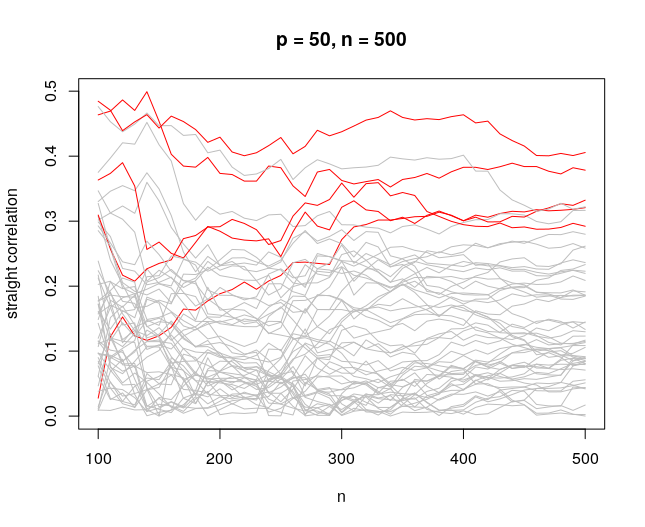
\includegraphics[width=\textwidth]{../plots/low-dim cor}
        \caption{}
    \end{subfigure}
    \begin{subfigure}[b]{0.45\textwidth}
        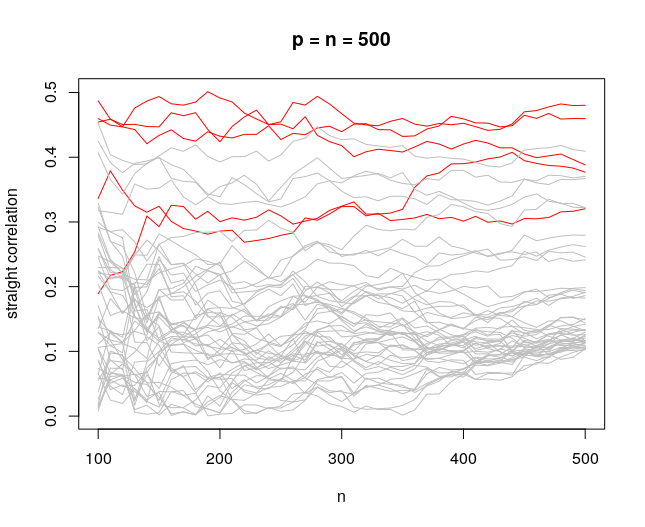
\includegraphics[width=\textwidth]{../plots/med-dim cor}
        \caption{}
    \end{subfigure}
    \begin{subfigure}[b]{0.45\textwidth}
        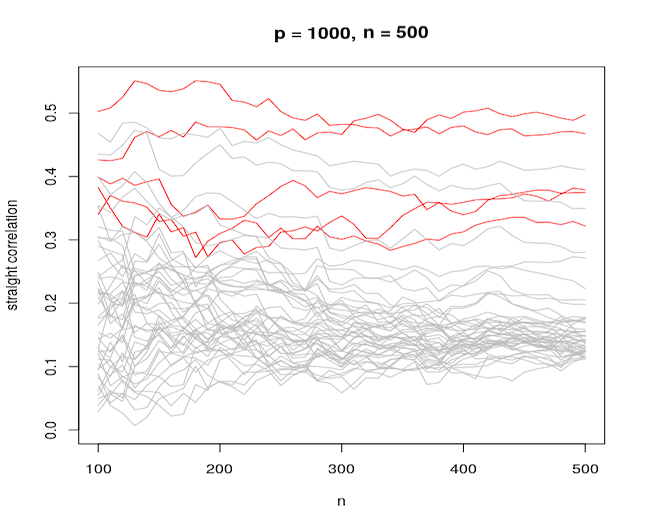
\includegraphics[width=\textwidth]{../plots/high-dim cor}
        \caption{}
    \end{subfigure}
    \begin{subfigure}[b]{0.45\textwidth}
        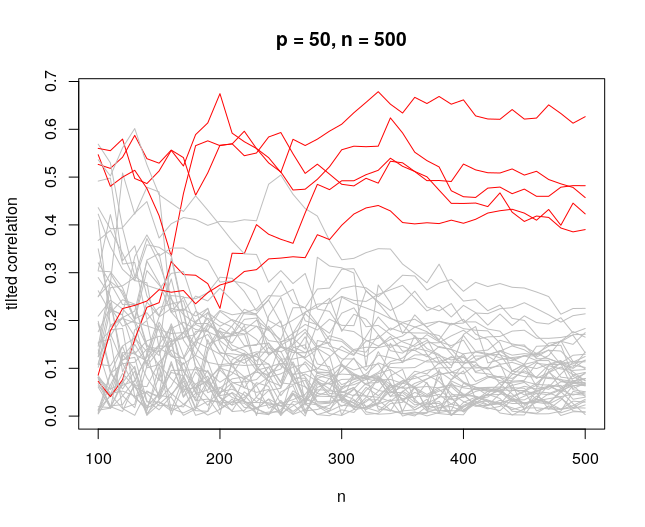
\includegraphics[width=\textwidth]{../plots/low-dim tilt}
        \caption{}
    \end{subfigure}
    \begin{subfigure}[b]{0.45\textwidth}
        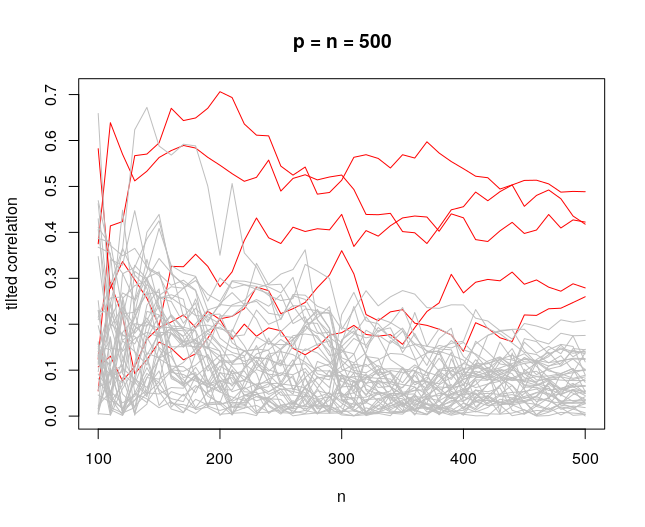
\includegraphics[width=\textwidth]{../plots/med-dim tilt}
        \caption{}
        \label{fig:tiger}
    \end{subfigure}
        \begin{subfigure}[b]{0.45\textwidth}
        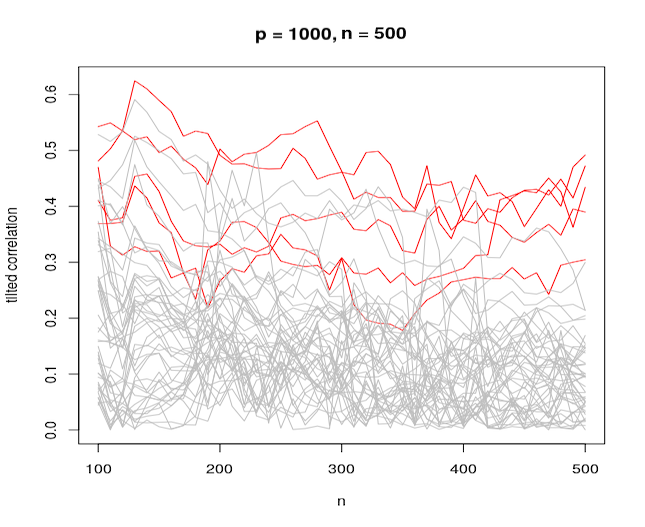
\includegraphics[width=\textwidth]{../plots/high-dim tilt}
        \caption{}
    \end{subfigure}
    \caption{Plots of absolute tilted and straight correlations for relevant predictors (red) along with 45 irrelevant predictors most correlated with the response (grey) against sample size. Plots (a)-(c) show straight correlations while (d)-(f) show tilted correlations.} \label{separation sim}
\end{figure}

\end{landscape}

\section{Efficient time series tilting}\label{efficient tilting}

The tilted correlation between the response variable and the j-th predictor is equivalent to the ordinary least squares estimate $\beta_{j}$ when regressing $y_t$ onto $\boldsymbol{x}_{t,\mathcal{D}_j}$ where $\mathcal{D}_j$ is the set $\left \{ \left \{ j \right \} \cup \mathcal{C}_j \right \}$. This implies a marginal regression model: 

\begin{equation*} \label{marginal model}
    Y = \mathbf{X}_{\mathcal{D}_j} \boldsymbol{\beta}_{\mathcal{D}_j} + \boldsymbol{u}_{\mathcal{D}_j}
\end{equation*}

Following the intuition from \textit{Section 4} of \cite{yousuf2018variable} observe that the error term in the marginal model is likely to be auto-correlated even if the error term in the full model is independently distributed. In this setting, by the main result in \cite{aitkin1935least}, a more efficient estimator in the MSE sense can be obtained by accounting for the serial correlation in the errors $\left \{ \left ( u_{t,\mathcal{D}_j} \right ) t \in \mathbb{Z} \right \}$.

\subsubsection{An in-feasible estimator}

Let $\Sigma_j$ be the $n \times n$ auto-covariance matrix for the unobservable errors $u_{1,\mathcal{D}_j},...,u_{n,\mathcal{D}_j}$. Then a vector of weighted predictors can be defined as $\widetilde{X}_j = \Sigma_j^{-\frac{1}{2}} X_j$, and an efficient estimator for the j-th tilted correlation is as follows: 

\begin{equation*}
    \widetilde{c_j^*}= \left ( \mathring{\widetilde{X}}_j^* \right )^T \mathring{\widetilde{Y}} / \left ( \mathring{\widetilde{X}}_j^T \left ( \mathbf{I} - \widetilde{\Pi}_j \right ) \mathring{\widetilde{X}}_j \right )
\end{equation*}

Clearly both $\widetilde{c_j^*}$ and $c_j^*$ converge in probability to the same object, hence the separation property also holds for $\widetilde{c_j^*}$. Since the latter is efficient in the MSE sense this suggests that the performance of the TCS algorithm will improve (or at the very least will not deteriorate) when $\widetilde{c_j^*}$ is used. 

\subsubsection{A feasible estimator}

Since $\Sigma_j$ is never observed $\widetilde{c_j^*}$ is in-feasible. Given any consistent estimator $\widehat{\Sigma}_j$ for $\Sigma_j$ a feasible estimate for the j-th tilted correlation is as follows: 

\begin{equation*}
    \widehat{c_j^*}= \left ( \mathring{\widehat{X}}_j^* \right )^T \mathring{\widehat{Y}} / \left ( \mathring{\widehat{X}}_j^T \left ( \mathbf{I} - \widehat{\Pi}_j \right ) \mathring{\widehat{X}}_j \right )
\end{equation*}

where $\widehat{X}_j = \widehat{\Sigma}_j^{-\frac{1}{2}} X_j$. Section \ref{efficiency proof} presents a proof for the equivalence of the limiting distribution of the feasible and in-feasible estimators. In addition to A\ref{A1}-A\ref{A9} the proof requires three assumptions listed below. If these conditions are met we can therefore expect the performance of the TCS algorithm to improve when $\widehat{c_j^*}$ is used. 

\subsubsection{Additional assumptions}

\begin{assump} \label{A10}
    The process $\left \{ \left ( y_t, \boldsymbol{x}_{t,\mathcal{D}_j}, \boldsymbol{u}_{t,\mathcal{D}_j} \right ), t \in \mathbb{Z} \right \}$ is a strictly stationary $\alpha$-mixing process with mixing coefficient given by A\ref{A7}. 
\end{assump}

\begin{assump} \label{A11}
    $\left \{ \left (u_{t,\mathcal{D}}  \right ) t \in \mathbb{Z} \right \}$ is a stationary AR$(p)$ process, where $p \in [0, Cn^{\theta})$ for some constant $C>0$.
\end{assump}

\begin{assump} \label{A12}
    The estimator $\widehat{\Sigma}_j$ is consistent in spectral norm, i.e. $ \mathbb{P} \left ( \left \| \widehat{\Sigma}_j - \Sigma_j \right \|_2 > \varepsilon \right ) \rightarrow 0$ as $n \rightarrow \infty$ for any $\varepsilon > 0$.
\end{assump}

Assumption A\ref{A10} follows naturally from assumption A\ref{A7}. Assumption A\ref{A11} imposes additional structure on $\Sigma_j$ which will be necessary to construct an estimator which converges to its population counterpart sufficiently fast. In practice the assumption is not too restrictive, as any stationary process with continuous spectral density  can be approximated arbitrarily well by a finite order linear AR process; see for example \textit{Corollary 4.4.2} in \cite{brockwell1991time}. Additionally, some structure will always need to be imposed on $\Sigma_j$ as the wholly unstructured problem requires the estimation of $n(n+1)/2$ parameters from a sample of only $n$ observations. 

Under A\ref{A11} the error term is of the form $u_{t,\mathcal{D}_j} + \sum_{k=1}^{p} \alpha_{k}(j) u_{t-k,\mathcal{D}_j} = e_{t,\mathcal{D}_j}$ with $e_{t,\mathcal{D}_j} \sim_{i.i.d} \mathcal{N}( 0,\omega_j^2 )$ for some constant $\omega_j>0$. An intuitive estimator $\widehat{\Sigma}_j$ can therefore be constructed by using residuals $\widehat{u}_{1,\mathcal{D}_j},...,\widehat{u}_{n,\mathcal{D}_j}$ from a first stage regression to estimate $\widehat{\alpha}_1(j),...,\widehat{\alpha}_p(j)$, whereupon the estimates are substituted into the $n \times n$ auto-covariance matrix for an AR(p) process. This type of parametric approach is popular in the econometric literature and has been shown to give efficient parameter estimates by \cite{amemiya1973generalized}, \cite{wickens1969consistency}, and \cite{koreisha2001generalized}, among others. Note that in practice the order of the AR process will be unknown; the order can be approximated by choosing the value of $p$ which minimises the AIC. 

Assumption A\ref{A12} requires that the estimator $\widehat{\Sigma}_j$ be more than point-wise consistent. This is necessary because in general point-wise consistency is not sufficient to guarantee that the feasible estimator will be more efficient than the least squares estimator; see for example the elegant counter-example in \textit{Section 2.5.12} of \cite{schmidt_1976}. In practice A\ref{A12} rules out the naive estimator $\widetilde{\Sigma}_j = \left ( \widehat{\gamma}_{|i-j|} \right )_{1\leq i,j \leq n}$ with $\widehat{\gamma}_k = \frac{1}{n}\sum_{t=1}^{n-|k|}\widehat{u}_{t,\mathcal{D}_j}\widehat{u}_{t+|k|,\mathcal{D}_j}$; as shown by \cite{wu2009banding} the largest eigenvalue of $\left ( \widetilde{\Sigma}_j - \Sigma_j \right )$ does not go to zero as the sample size goes to infinity, hence the estimator cannot be consistent in spectral norm. 

\subsection{Proof of efficiency} \label{efficiency proof}

\bigskip

\fbox{
\begin{minipage}{\columnwidth}
    \begin{theorem} \label{efficiency theorem}
    For the j-th tilted correlation, under assumptions A\ref{A1}-A\ref{A12} and using the intuitive estimator suggested in Section \ref{efficient tilting} it holds that:
    
    \begin{equation*}
        \sqrt{n}\left ( \widehat{c_j^*}- \beta_{(j)} \right ) \rightarrow_d \sqrt{n}\left ( \widetilde{c_j^*}- \beta_j_{(j)} \right )
    \end{equation*}
    
    \end{theorem}
\end{minipage}
}

\bigskip

\textbf{Proof:}

By \textit{Theorem 15} in \cite{schmidt_1976} sufficient conditions for the feasible and in-feasible tilted correlations to have the same limiting distribution are the following:

\begin{align*}
    & \lim_{n \rightarrow \infty}\mathbb{P}\left ( \Delta_3 \right ) := \lim_{n \rightarrow  \infty}\mathbb{P}\left ( \frac{1}{n}\left | X_j^T\left ( \widehat{\Sigma }_j^{-1} - \Sigma_j^{-1} \right )X_j  \right | > \varepsilon \right ) = 0 \\
    & \lim_{n \rightarrow  \infty}\mathbb{P}\left ( \Delta_4 \right ) :=  \lim_{n \rightarrow \infty}\mathbb{P}\left ( \frac{1}{\sqrt{n}}\left | X_j^T\left ( \widehat{\Sigma }_j^{-1} - \Sigma_j^{-1} \right )\boldsymbol{\epsilon}_\mathcal{D}  \right | > \varepsilon \right ) = 0 
\end{align*}
 
\bigskip
 
where $\varepsilon>0$ is a small positive constant. To show that $\mathbb{P}(\Delta_3)$ gos to zero it will be useful to have some link between convergence of $\widehat{\Sigma}_j$ in spectral norm as guaranteed by A\ref{A12} and convergence of the inverse. Such a link is provided by the following argument, which is taken from the proof of \textit{Theorem 3} in \cite{yousuf2018variable}. Let $a_1 \geq a_2 \geq ... \geq a_n $ be the ordered eigenvalues of the matrix $\Sigma_j^{-\frac{1}{2}}\widehat{\Sigma}_j\Sigma_j^{-\frac{1}{2}}$. Using the eigenvalue-norm inequality, see for example \textit{Proposition 4.4} in \cite{gallier}, we have that: 

\begin{align*}
    \lambda_{\min}\left ( \Sigma_j \right ) \left \| \widehat{\Sigma}_j^{-1} - \Sigma_j\right \|_2 & \leq \left \| \Sigma_j^{\frac{1}{2}}\left ( \widehat{\Sigma}_j^{-1} - \Sigma_j^{-1} \right )\Sigma_j^{\frac{1}{2}} \right \|_2 \\ 
    & = \left \| \Sigma_j^{\frac{1}{2}}\widehat{\Sigma}_j^{-1}\Sigma_j^{\frac{1}{2}} - \mathbf{I}_n \right \|_2 \\
    & = \max_{i \leq n}\left | \frac{1-a_i}{a_i} \right |
\end{align*}

Going in the other direction we have that: 

\begin{align*}
    \max_{i \leq n}\left | a_i - 1 \right | & = \left \| \Sigma_j^{-\frac{1}{2}} \widehat{\Sigma}_j \Sigma_j^{-\frac{1}{2}} - \mathbf{I}_n \right \|_2 \\
    & \leq \lambda_{\max} (\Sigma_j^{-1} )\left \| \widehat{\Sigma}_j - \Sigma_j \right \|_2
\end{align*}

Finally, define $a_j = \min_{i \leq n} \left | a_i^{-1} \right |$. By assumption A\ref{A11} the eigenvalues of $\Sigma_j$ are guaranteed to be bounded away from zero and infinity, and the link is therefore valid. This is because the spectral density of a finite order AR process is bounded away from zero and infinity. Using the fact that with standardised and de-meaned entries $\left \| X_j \right \|_2^2 = n$ we have that: 

\begin{align*}
    \mathbb{P}\left ( \Delta_3 \right ) & \leq \mathbb{P}\left ( \left \| \widehat{\Sigma}_j^{-1} - \Sigma_j^{-1} \right \|_2 > \varepsilon \right ) \\
    & \leq \mathbb{P}\left ( \max_{i \leq n}\left | \frac{1-a_i}{a_i} \right | > \varepsilon' \right ) \\
    & \leq \underbrace{\mathbb{P}\left ( \left \| \widehat{\Sigma}_j - \Sigma_j \right \|_2 > \varepsilon''/M_\varepsilon \ \right )}_5 + \underbrace{\mathbb{P}\left ( a_j < M_\varepsilon \right )}_6
\end{align*}

By setting $M_\varepsilon = 1 - \varepsilon$ convergence of term 5 is guaranteed under assumption A\ref{A12}. Convergence of term 6 can be shown through its connection to the spectral norm of the approximation error as follows:  

\begin{align*}
    \mathbb{P}\left ( a_j < M_\varepsilon \right ) & \leq \mathbb{P}\left ( \left | a_j -1  \right | > M_\varepsilon - 1 \right ) \\ 
    & = \mathbb{P}\left ( \max_{i \leq n}\left | a_i -1 \right | > \varepsilon \right ) \\
    & \leq \mathbb{P}\left ( \left \| \widehat{\Sigma}_j - \Sigma_j \right \|_2 > \varepsilon '\right )
\end{align*}

To show $\mathbb{P}\left ( \Delta_4 \right )$ goes to zero we can make use of the additional structure provided by assumption A\ref{A10}. The next argument closely follows the proof of \textit{Condition 3.10} in \cite{wickens1969consistency}. Note that the error terms can be can be expressed in matrix form as $\boldsymbol{Ju}_{\mathcal{D}_j} = \boldsymbol{e}^*$, where $e_{t,\mathacal{D}_j}^*$ is defined as $e_{t,\mathacal{D}_j} - \sum_{s=t-p}^{0} \alpha_{t-s}(j) u_{s,\mathcal{D}_j}$ for $t \leq p$ and $e_{t,\mathacal{D}_j}$ otherwise, and $\boldsymbol{J} = \boldsymbol{I}_n + \alpha_1(j)\boldsymbol{L} + ...+ \alpha_p(j)\boldsymbol{L}^p$  with $\boldsymbol{L}$ being an augmented $\boldsymbol{0}_{n \times n}$ matrix given by:

\begin{equation*}
    \boldsymbol{L} = \begin{pmatrix}
    0 & \boldsymbol{I}_{n-1}\\ 
    0 & 0
    \end{pmatrix}
\end{equation*}

It therefore follows that: 

\begin{align*}
    \mathbb{E}\left ( \boldsymbol{Ju}_{\mathcal{D}_j}\left ( \boldsymbol{Ju}_{\mathcal{D}_j} \right )^T \right ) & = \boldsymbol{J}\mathbb{E}\left ( \boldsymbol{u}_{\mathcal{D}_j}\boldsymbol{u}_{\mathcal{D}_j}^T \right ) \boldsymbol{J}^T \\ 
    & = \boldsymbol{J} \Sigma_j \boldsymbol{J}^T\\ 
    & = \omega_j^2 \begin{pmatrix}
    \boldsymbol{I}_{n-p} & \boldsymbol{0} \\ 
    \boldsymbol{0} & \boldsymbol{G}
    \end{pmatrix}
\end{align*}

where $\boldsymbol{G}$ is a $p \times p$ positive definite matrix. Using the above, the inverse auto-covariance matrix can be written as: 

\begin{equation*}
    \Sigma_j^{-1} = \omega_j^{-2} \boldsymbol{J}^T \begin{pmatrix}
    \boldsymbol{I}_{n-p} & \boldsymbol{0} \\ 
    \boldsymbol{0} & \boldsymbol{G}^{-1}
    \end{pmatrix} \boldsymbol{J}
\end{equation*}
    
Let a wide-hat indicate that AR coefficients have been replaced by consistent sample estimates. As long as $\widehat{\omega}_j^{-2}$ is consistent for $\omega_j^{-2}$ we have that $\left ( \widehat{\Sigma}_j^{-1}-\Sigma_j^{-1} \right )$ in $\Delta_4$ can be replaced with $\left ( \widehat{\Sigma}_j^*-\Sigma_j^* \right )$ where the relevant matrices are defined below: 

\begin{align*}
    \Sigma_j^* & = \boldsymbol{J}^T \begin{pmatrix}
    \boldsymbol{I}_{n-p} & \boldsymbol{0} \\ 
    \boldsymbol{0} & \boldsymbol{G}^{-1}
    \end{pmatrix} \boldsymbol{J} \\
    & \\
    \widehat{\Sigma}_j^* & = \widehat{\boldsymbol{J}}^T \begin{pmatrix}
    \boldsymbol{I}_{n-p} & \boldsymbol{0} \\ 
    \boldsymbol{0} & \widehat{\boldsymbol{G}}^{-1}
    \end{pmatrix} \widehat{\boldsymbol{J}}
\end{align*}

Partitioning $\boldsymbol{J}^T = \left ( \boldsymbol{J}_1^T, \boldsymbol{J}_2^T \right )$ and $\widehat{\boldsymbol{J}}^T = \left ( \widehat{\boldsymbol{J}}_1^T, \widehat{\boldsymbol{J}}_2^T \right )$, where the first sub-matrix has dimensions $(n-p) \times n$ and the second has dimensions $p \times n$, the left hand side of event $\Delta_4$ can then be re-written as the following: 

\begin{align*}
    \frac{X_j\left ( \widehat{\Sigma}_j^* - \Sigma_j^* \right ) \boldsymbol{u}_{\mathcal{D}_j}}{\sqrt{n}} & = \underbrace{n^{-\frac{1}{2}}X_j^T \widehat{\boldsymbol{J}}_2^T \left ( \widehat{\boldsymbol{G}}^{-1}-\boldsymbol{I}_p \right )\widehat{\boldsymbol{J}}^T_2 \boldsymbol{u}_{\mathcal{D}_j} - n^{-\frac{1}{2}}X_j^T \boldsymbol{J}_2^T \left ( \boldsymbol{G}^{-1}-\boldsymbol{I}_p \right )\boldsymbol{J}^T_2 \boldsymbol{u}_{\mathcal{D}_j}}_7 \\
    & + \underbrace{n^{-\frac{1}{2}}X_j^T\left ( \widehat{\boldsymbol{J}} - \boldsymbol{J} \right )^T\left ( \widehat{\boldsymbol{J}} - \boldsymbol{J} \right ) \boldsymbol{u}_{\mathcal{D}_j}}_{8} \\
    & + \underbrace{n^{-\frac{1}{2}}X_j^T\left ( \widehat{\boldsymbol{J}} - \boldsymbol{J} \right )^T\boldsymbol{J} \boldsymbol{u}_{\mathcal{D}_j}}_9 + \underbrace{n^{-\frac{1}{2}}X_j^T \boldsymbol{J}^T\left ( \widehat{\boldsymbol{J}} - \boldsymbol{J} \right )^T \boldsymbol{u}_{\mathcal{D}_j}}_{10}
\end{align*}

A sequence of random variables $\left \{ a_n \right \}_{n=1}^\infty$ is said to be $\mathcal{O}_p(b_n)$, where  $\left \{ b_n \right \}_{n=1}^\infty$ is a deterministic sequence, if for any $\varepsilon >0$ there exist constants $c>0$ and $n_0 > 0$ such that $\mathbb{P}\left ( \left | a_n \right | > c \cdot b_n \right )< \varepsilon$ whenever $n \geq n_0$. By the specialised form of the $\boldsymbol{G}$ matrix, and the element-wise consistence of $\widehat{\boldsymbol{J}}$ and $\widehat{\boldsymbol{G}}$, term 7 is at least $\mathcal{O}_p(n^{-\frac{1}{2}})$. By the central term being in quadratic form, term 8 goes to zero as long as $\left ( \widehat{\alpha}_s(j) - \alpha_s(j) \right ) = \mathcal{O}_p(n^{-\frac{1}{2}})$ for each $s \in [1,p]$, which is a condition generally satisfied by consistent estimators. Finally, terms 9 and 10 involve $p^2$ sums of the form $\alpha_s(j)\left ( \widehat{\alpha}_r(j) - \alpha_r(j) \right )\times n^{-\frac{1}{2}} \left ( \boldsymbol{L}^rX_j \right )^T \boldsymbol{L}^s\boldsymbol{u}_{\mathcal{D}_j}}$ for $r,s \in [1,p]$. The desired result therefore holds whenever $n^{-\frac{1}{2}}\left ( \boldsymbol{L}^rX_j \right )^T \boldsymbol{L}^s\boldsymbol{u}_{\mathcal{D}_j}} = \mathcal{O}_p(1)$, which is clearly the case under assumption A\ref{A10}. 

\section{Stable time series tilting} \label{stable tilting}

Construction of the set $\mathcal{C}_j$ is crucial to the performance of the TCS algorithm. Both the number of predictors incorrectly included in $\mathcal{C}_j$ (the false positives - FP) and the number incorrectly excluded from the set (the false negatives - FN) will reduce the effectiveness of the tilted correlation as a screening device. In Section \ref{tilting introduction} it was proposed that the choice of $\pi_{n}$ controls the expected FDR at $p_n^{-\frac{1}{2}}$; this can be improved by choosing a larger $\pi_{n}$, hover a fall in the type I error necessitates a trade-off in terms of the type II error. In this section I propose a re-sampling approach based on the work of \cite{meinshausen2010stability} which, for a given $\pi_{n}$, seeks to reduce the number of false positives with minimal impact on the number of false negatives. 

\subsubsection{Primer on stability selection}

The stability selection of \cite{meinshausen2010stability} is a wrap-around procedure designed to enhance any feature screening algorithm that selects a subset of features, say $\widehat{\mathcal{S}}$, via regularisation. The authors point out that choosing the right amount of regularisation is often extremely difficult. Stability selection uses a grid of regularisation parameters $\Lambda$ and a set of pseudo samples $\boldsymbol{Z}^*_1,...,\boldsymbol{Z}^*_N$ obtained by randomly sampling $n/2$ observations from the original data without replacement (i.e. sub-sampling). Let $\widehat{\mathcal{S}}_i^{\lambda}$ be the set of features selected by the base algorithm using pseudo-sample $\boldsymbol{Z}_i^*$ under some level of regularisation $\lambda$. For each feature $k$ the selection probability under $\lambda \in \Lambda$ is calculated as $\widehat{\Pi}_k^{\lambda} = \frac{1}{N}\sum_{i=1}^{N}\mathcal{I}\left ( k \in \widehat{\mathcal{S}}_i^{\lambda} \right )$, where $\mathcal{I}(\cdot)$ is the indicator function. The set of stable features is then defined as follows:

\begin{equation*}
    \widehat{\mathcal{S}}^{\text{stable}} = \left \{ k:\max_{\lambda \in \Lambda} \left( \widehat{\Pi}^{\lambda}_k \right ) \geq \upsilon_{th}  \right \} 
\end{equation*}

Intuitively, stability selection injects noise into the original data by re-sampling, and selects only those features which survive the screening process with high probability. The authors claim that stability selection works well for any choice of $\upsilon_{th}$ in the interval $(0.6,0.9)$. A theorem is also provided which bounds the expected number of falsely selected features (the family-wise type I error - FWE) based on the choice of $\upsilon_{th}$, however this requires knowledge of the average number of features selected by the base algorithm. 

\subsubsection{Extension to stable tilting}

Here I introduce stable tilting, in which for each predictor a `stable' conditioning set $\mathcal{C}_j^{stb}$ is constructed according to the principle of stability selection. The procedure begins with calculating $\pi_{n}$ using the original sample. A grid of thresholds is therefore defined as $\Lambda = \left \{ \pi_{(1)},...,\pi_{(G)} \right \}$, with $\pi_{n} = \pi_{(1)}< \pi_{(2)}<...<\pi_{(G)} = c \cdot \pi_{n}$ for some $c \gg 1$. In keeping with stability selection pseudo-samples $\boldsymbol{X}_1^*,...,\boldsymbol{X}_N^*$ are generated from the original sample, and a stable conditioning set for the j-th predictor is constructed according to $\mathcal{C}_j^{stb} = \left \{ k : \max_{\pi \in \Lambda}\left ( \widehat{\Pi}_k^{\pi} \right ) \geq \upsilon_{th} \right \}$. Figure \ref{stable tilting fig} provides a graphical representation of the procedure. 

\begin{figure}[H]
    \centering
    \includegraphics[width = \textwidth]{../plots/stable tilting visualised}
    \caption{Diagram of stable tilting being used to construct a set of highly correlated predictors for the j-th predictor.}
    \label{stable tilting fig}
\end{figure}

The construction of $\Lambda$ ensures that for each pseudo-sample $\boldsymbol{X}_i^*$ and for every $\pi \in \Lambda$ the highest expected FDR is around $p_n^{-\frac{1}{2}}$, and in general will be smaller. Since selection is made on the basis of the highest selection probability among all thresholds, we can expect predictors which are correlated at the population level to survive the screening process. Meanwhile, predictors which attain a high correlation spuriously are less likely to do so over multiple pseudo-samples. A more refined approach would involve re-calculating $\pi_{n}$ for each pseudo-sample to ensure the expected FRD is exactly $p_n^{-\frac{1}{2}}$. This however is computationally expensive, and simulation studies confirm that in practice the difference in selected variables is negligible.  

The original stability selection procedure was developed for $\text{i.i.d.}$ data. To adapt to the time series setting I suggest generating $\boldsymbol{X}_1^*,...,\boldsymbol{X}_N^*$ using the stationary bootstrap described in Section \ref{Bootstrapping ts} as the method is well suited to replicating the dependence structure in stationary time series. Sub-sampling can also be used to generate pseudo samples from stationary time series using blocks of data, see \textit{Chapters 2-3} of \cite{politis1999subsampling} for a detailed explanation. However, there is very little literature on using random block sizes to preserve strict stationarity as in the case of the stationary bootstrap. Additionally, there are subtle differences between the two procedures: sub-sampling treats each block as its own ``mini time series'' whereas the bootstrap uses blocks as ``building stones to construct a new pseudo time series''; see \textit{Section 3.9} of  Politis et al. for a comparison. In the context of selecting a stable conditioning set, the latter seems preferable. In the i.i.d. setting Meinshausen and Bühlmann opt for sub-samples of size $n/2$ as they ``resembles most closely the bootstrap while allowing computationally efficient implementation''. However open source implementations of stability selection in the R and Python communities, see for example \cite{Huijskens0stability}, allow for the use of the bootstrap as in practice the computational gains from sub-sampling in terms or run-time are modest - this further supports the use of the stationary bootstrap.

Finally, I note that stable tilting can be seen as a first step in addressing Professor Howell Tong's question raised in the discussion section of \cite{meinshausen2010stability}, namely whether stability selection may be used in time series modelling. This question, to my knowledge, has not yet been explored in the literature. 

\subsection{Simulation study}\label{stability simulation}

To illustrate the effect of stable tilting on membership of the conditioning set I present the following three simulation studies. Here the idea is to show that stable tilting can be used to construct a more parsimonious conditioning set than tilting alone. In each simulation the sample size was fixed at $n=500$ and the number of predictors was varied over $p=\left \{ 50,500,1000 \right \}$. For ease of comparison I focus on $\mathcal{C}_1$, the conditioning set for the first predictor. To construct a stable conditioning set $N=50$ bootstrap replicates were generated using the stationary bootstrap of \cite{politis1994stationary} with the average block size set to $l_n = 25$, and $v_{th}$ was set to $0.6$. 

\subsubsection{Simulation no. 1}

Data was generated according to a VAR(1) process given by $\mathbf{x}_t = \Phi \mathbf{x}_{t-1} + \boldsymbol{\nu}_t$ as in Section \ref{separation sim explained}. The vector of innovations was generated according to $\boldsymbol{\nu}_t \sim_{i.i.d} \mathcal{N}_p\left ( \mathbf{0}, \Sigma \right )$ where $\Sigma = \left \{ \rho^{|i-j|} \right \}_{i,j \leq p}$ and $\rho$ was varied over $\left \{ 0.7,0.8,0.9 \right \}$. The first row of $\Sigma$ was replaced by the vector $\left ( 1,0,...,0 \right )$. The coefficient matrix was set to $\Phi = \textit{diag}\left ( 0.4 \right )$ and the first row was replaced by a zero vector with the first $10$ entries set to $0.5$. 

We can express $x_{t,1} = 0.5\sum_{k=2}^{10}x_{t,k} +\nu_{t,1}$, and conditional on the set $\mathcal{C}_1^*=\left \{ 2,...,10 \right \}$ predictor one is independent of the remaining predictors. I therefore count a false negative as excluding a member of $\mathcal{C}_1^*$ and a false positive as including a member of $\mathcal{J} \setminus\left \{ \mathcal{C}_1^* \cup \left \{ 1 \right \} \right \}$. Clearly, not accounting for $\mathcal{C}_1^*$ predictor one is correlated with every other predictor. The test is therefore more challenging than the setting described in Section \ref{stable tilting}, where the aim was simply to filter out uncorrelated predictors. 

\subsubsection{Simulation no. 2}

The setup is identical to the previous simulation, with the additional condition that each predictor is observed with additive $\text{i.i.d.}$ $\mathcal{N}(0,3)$ noise. This replicates the realistic scenario in which a time series is observed with some non-systematic measurement error. Since the variance of the contaminating noise is nine times larger than that of marginal innovation in the VAR process, this setting is considerably more challenging than the last. 

\subsubsection{Simulation no. 3}

The setup is identical to the first simulation, with the exception that the first row of $\Phi$ is instead replaced by a zero vector where the first entry along with nine more entries spaced maximally apart are set to $0.5$. For example, with $p=500$ the set of predictors we aim to identify is $\mathcal{C}_1^*=\left \{ 56,112, 167, 223, 278, 334, 389, 445, 500 \right \}$. This setting is more challenging than the previous simulations: where predictors in $\mathcal{C}_j^*$ were highly correlated among themselves and weakly correlated with irrelevant predictors, now predictors in the target set are attain the minimal possible correlation among themselves and are highly correlated with `irrelevant' predictors. 

\subsubsection{Simulation results}

Simulation results are reported in Tables \ref{stabsim1}, \ref{stabsim2}, and \ref{stabsim3}, where FP and FN were calculated as the the average of 100 trials. The improved performance of stable tilting is immediately clear: in each scenario stable tilting achieves a lower value for FP+FN than tilting alone. The result is driven, as expected, by the fact that stable tilting commits far fewer type II errors. stable tilting does tends to commit slightly more type I errors; this is because using a grid of parameters on bootstrap samples destroys the expected FDR control enjoyed by the original procedure. However, for sufficiently large $\rho$ the effect is negligible. This suggests that the new procedure will work best when the design matrix is highly correlated. All things being equal increasing the number of predictors has a greater effect on the number of type II errors committed, suggesting the new procedure should be used when $p_n$ is large. Finally, it should be noted that stable tilting is highly computationally intensive. With the parameters chosen in these simulation each $\mathcal{C}_1^{stb}$ is around 1,000 times more expensive to compute than $\mathcal{C}_1$. Since the TCS algorithm computes $\mathcal{O}(m \cdot n^\xi)$ tilted correlations, stable tilting should only be used when it is suspected that doing so will improve significantly the performance of the TCS algorithm. 

\newpage
\begin{landscape}
\begin{table}
\begin{tabular}{|c|cccccc|cccccc|cccccc|cccccc}
\multicolumn{1}{c}{} & \multicolumn{6}{c}{(p = 50)} & \multicolumn{6}{c}{(p = 500)} & \multicolumn{6}{c}{(p = 1,000)} \\
\cmidrule(r){2-19}
\multicolumn{1}{c}{} & \multicolumn{3}{c}{Tilting} & \multicolumn{3}{c}{Stability} & \multicolumn{3}{c}{Tilting} & \multicolumn{3}{c}{Stability} & \multicolumn{3}{c}{Tilting} & \multicolumn{3}{c}{Stability}\\
\cmidrule(r){2-19}
$\rho$  &   FP  & FN & FP+FN & FP  & FN & FP+FN &   FP  & FN & FP+FN & FP  & FN & FP+FN & FP  & FN & FP+FN & FP  & FN & FP+FN \\
\hline
0.7 & $1.9$ & $0.6$ & $2.5$ & $1.3$ & $1.1$ & $\boldsymbol{2.4}$ & $63.1$ & $0.1$ & $63.2$ & $43.0$ & $0.3$ & $\boldsymbol{43.2}$ & $238.0$ & $0.1$ & $238.1$ & $211.0$ & $0.2$ & $\boldsymbol{211.1}$ \\
0.8 & $3.3$ & $0.2$ & $3.5$ & $2.1$ & $0.4$ & $\boldsymbol{2.5}$ & $63.1$ & $0.0$ & $63.1$  & $44.1$ & $0.1$ & $\boldsymbol{44.2}$ & $244.9$ & $0.0$ & $244.9$ & $219.4$ & $0.0$ & $\boldsymbol{219.4}$ \\
0.9 & $7.6$ & $0.0$ & $7.6$ & $5.9$ & $0.0$ & $\boldsymbol{5.9}$ & $71.8$ & $0.0$ & $71.8$ & $52.3$ & $0.0$ & $\boldsymbol{52.3}$ & $244.6$ & $0.0$ & $244.6$ & $215.3$ & $0.0$ & $\boldsymbol{215.3}$  \\
\hline
\end{tabular}
\caption{Screening accuracy of tilting versus stabilised tilting for the set $\mathcal{C}_1$ with nine consecutive relevant predictors in a VAR(1) setting; lowest values for FP+FN are in bold.}
\label{stabsim1}
\end{table}

\begin{table}
\begin{tabular}{|c|cccccc|cccccc|cccccc|cccccc}
\multicolumn{1}{c}{} & \multicolumn{6}{c}{(p = 50)} & \multicolumn{6}{c}{(p = 500)} & \multicolumn{6}{c}{(p = 1,000)} \\
\cmidrule(r){2-19}
\multicolumn{1}{c}{} & \multicolumn{3}{c}{Tilting} & \multicolumn{3}{c}{Stability} & \multicolumn{3}{c}{Tilting} & \multicolumn{3}{c}{Stability} & \multicolumn{3}{c}{Tilting} & \multicolumn{3}{c}{Stability}\\
\cmidrule(r){2-19}
$\rho$  &   FP  & FN & FP+FN & FP  & FN & FP+FN &   FP  & FN & FP+FN & FP  & FN & FP+FN & FP  & FN & FP+FN & FP  & FN & FP+FN \\
\hline
0.7 & $1.9$ & $0.6$ & $2.5$ & $1.1$ & $1.3$ & $\boldsymbol{2.4}$ & $58.7$ & $0.2$ & $58.8$ & $40.2$ & $0.3$ & $\boldsymbol{40.5}$ & $230.5$ & $0.1$ & $230.6$ & $202.2$ & $0.2$ & $\boldsymbol{202.4}$  \\
0.8 & $3.2$ & $0.2$ & $3.4$ & $2.4$ & $0.3$ & $\boldsymbol{2.7}$ & $59.7$ & $0.0$ & $59.7$ & $39.1$ & $0.1$ & $\boldsymbol{39.2}$ & $232.7$ & $0.0$ & $232.7$ & $203.1$ & $0.0$ & $\boldsymbol{203.1}$ \\
0.9 & $7.5$ & $0.0$ & $7.6$ & $5.7$ & $0.1$ & $\boldsymbol{5.8}$ & $69.2$ & $0.0$ & $69.2$ & $49.2$ & $0.0$ & $\boldsymbol{49.2}$ & $238.2$ & $0.0$ & $238.2$ & $210.1$ & $0.0$ & $\boldsymbol{210.1}$ \\
\hline
\end{tabular}
\caption{Screening accuracy in a VAR(1) setting with nine consecutive relevant predictors where each predictor is observed with noise; lowest values for FP+FN are in bold.}
\label{stabsim2}
\end{table}

\begin{table}
\begin{tabular}{|c|cccccc|cccccc|cccccc|cccccc}
\multicolumn{1}{c}{} & \multicolumn{6}{c}{(p = 50)} & \multicolumn{6}{c}{(p = 500)} & \multicolumn{6}{c}{(p = 1,000)} \\
\cmidrule(r){2-19}
\multicolumn{1}{c}{} & \multicolumn{3}{c}{Tilting} & \multicolumn{3}{c}{Stability} & \multicolumn{3}{c}{Tilting} & \multicolumn{3}{c}{Stability} & \multicolumn{3}{c}{Tilting} & \multicolumn{3}{c}{Stability}\\
\cmidrule(r){2-19}
$\rho$  &   FP  & FN & FP+FN & FP  & FN & FP+FN &   FP  & FN & FP+FN & FP  & FN & FP+FN & FP  & FN & FP+FN & FP  & FN & FP+FN \\
\hline
0.7 & $8.7$ & $5.3$ & $14.0$ & $5.5$ & $6.4$ & $\boldsymbol{12.0}$ & $66.o$ & $3.8$ & $69.8$ & $45.4$ & $4.8$ & $\boldsymbol{50.2}$ & $243.0$ & $2.7$ & $245.7$ & $214.9$ & $3.4$ & $\boldsymbol{218.3}$ \\
0.8 & $17.6$ & $3.8$ & $21.4$ & $13.0$ & $5.0$ & $\boldsymbol{18.0}$ & $77.0$ & $3.6$ & $80.6$ & $53.6$ & $4.6$ & $\boldsymbol{58.2}$ & $250.7$ & $2.5$ & $253.2$ & $223.0$ & $3.2$ & $\boldsymbol{226.2}$ \\
0.9 & $31.5$ & $1.6$ & $33.1$  & $27.5$ & $2.5$ & $\boldsymbol{30.0}$ & $96.4$ & $3.8$ & $100.2$ & $68.4$ & $4.7$ & $\boldsymbol{73.1}$  & $271.9$ & $2.6$ & $274.5$ & $238.3$ & $3.3$ & $\boldsymbol{241.6}$ \\
\hline
\end{tabular}
\caption{Screening accuracy in a VAR(1) setting with nine maximally spaced relevant predictors (observed without noise); lowest values for FP+FN are in bold.}
\label{stabsim3}
\end{table}
\end{landscape}

\chapter{Numerical Studies} \label{numerical}

\section{Extended simulation studies}\label{extended simulation studies}

In this section simulation studies are used to compare the screening accuracy of the TCS algorithm executed with standard tilted correlations against that of same algorithm executed with extensions proposed in Sections \ref{efficient tilting} and \ref{stable tilting}. For each simulation data was generated according to a VAR(1) process given by $\mathbf{x}_t = \Phi \mathbf{x}_{t-1} + \boldsymbol{\nu}_t$ as in Section \ref{separation sim explained}. Similarly the response variable was generated according to $y_t = \boldsymbol{\beta}^T\mathbf{x}_t + e_t$ where $e_t$ followed an AR(1) process, and the five non-zero entries in $\boldsymbol{\beta}$ were set to either $-1$ or $1$. Each time the TCS algorithm was run the stopping index was set to $m=20$. Stable tilted correlations were estimated as set out in Section \ref{stability simulation}. For ease of comparison results are presented in the form of Receiver Operator Characteristic (ROC) curves, which plot the True Positive Rate (TPR) against the False Positive Rate (FPR).

\subsection{General comparison of screening performance}\label{general comparison}

For a general comparison of the three methods I first consider a setting which conforms to assumptions A\ref{A1}-A\ref{A12}, and record the effect of varying the population noise level and sample size. In keeping with \textit{Section 4} of \cite{cho2012high} the noise level is quantified via $R^2 = \mathbb{V}\left ( \boldsymbol{\beta}^T\mathbf{x}_t \right ) / \mathbb{V}\left ( y_t \right )$, where $\mathbb{V}(\cdot)$ gives the population variance. To gauge sensitivity to low sample sizes the number of predictors was held constant at $p=1,000$ and the sample size was varied over $n =\left \{ 500,200,100 \right \}$. In addition, to gauge sensitivity to the noise level innovations in the AR(1) process were drawn from $\mathcal{N}(0,r^2)$ and $r$ was varied in order to attain $R^2= \left \{ 0.9,0.6,0.3 \right \}$.  

\begin{figure}[h]
    \centering
    \begin{subfigure}[b]{0.3\textwidth}
        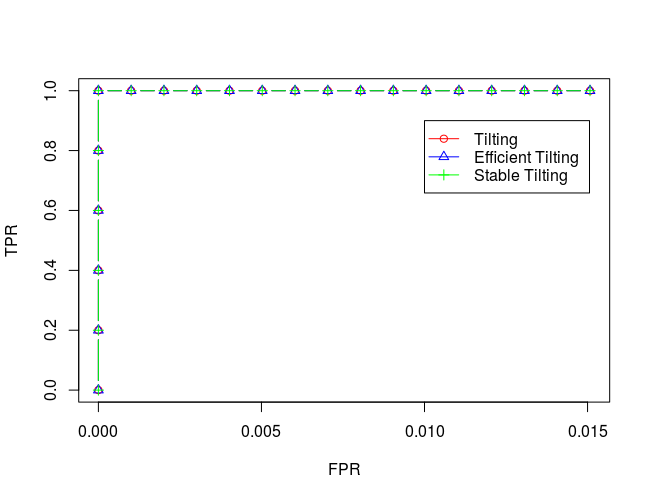
\includegraphics[width=\textwidth]{../plots/general09}
        \caption{}
    \end{subfigure}
    \begin{subfigure}[b]{0.3\textwidth}
        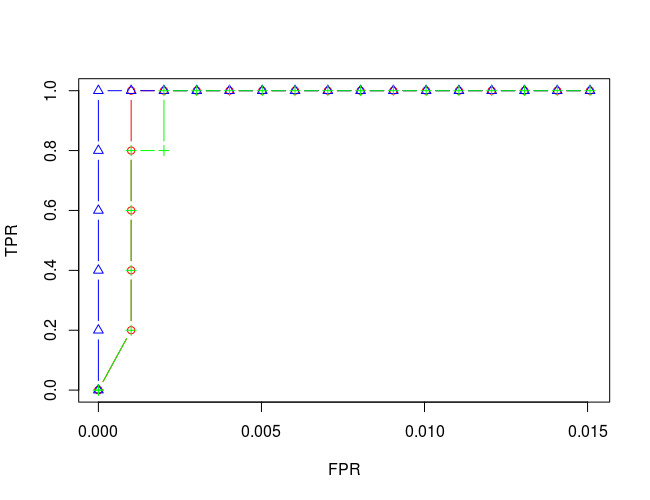
\includegraphics[width=\textwidth]{../plots/general06}
        \caption{}
    \end{subfigure}
    \begin{subfigure}[b]{0.3\textwidth}
        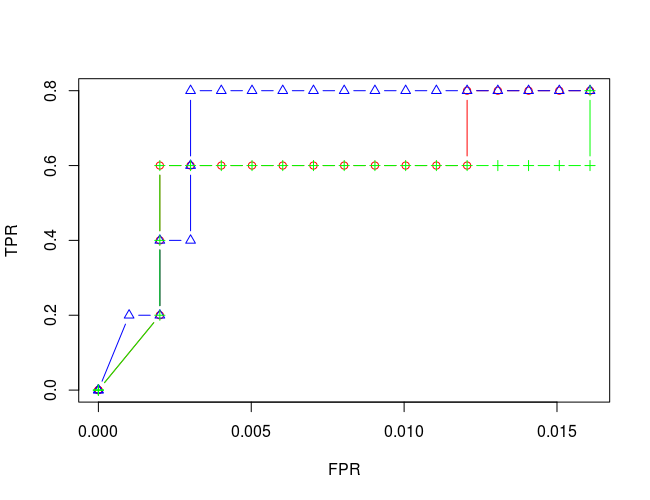
\includegraphics[width=\textwidth]{../plots/general03}
        \caption{}
    \end{subfigure}
    \begin{subfigure}[b]{0.3\textwidth}
        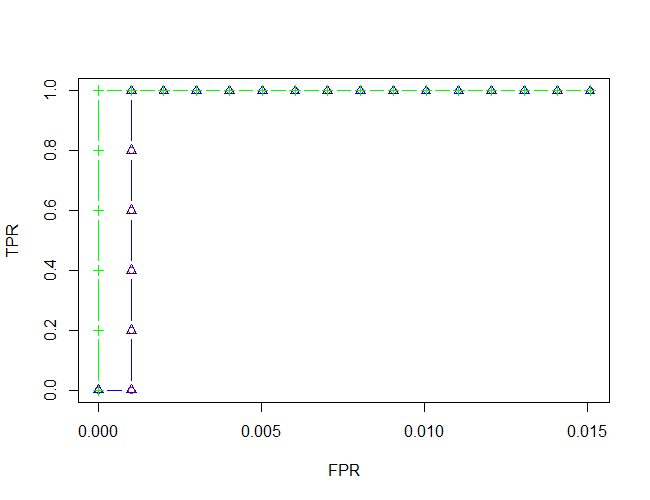
\includegraphics[width=\textwidth]{../plots/100sample09}
        \caption{}
    \end{subfigure}
    \begin{subfigure}[b]{0.3\textwidth}
        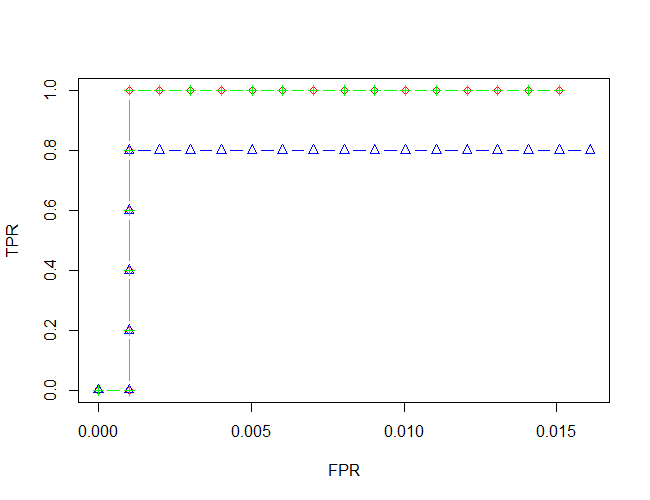
\includegraphics[width=\textwidth]{../plots/100sample06}
        \caption{}
    \end{subfigure}
    \begin{subfigure}[b]{0.3\textwidth}
        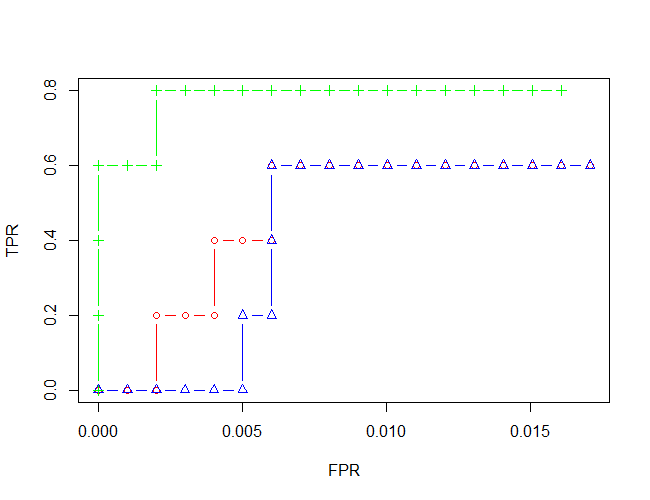
\includegraphics[width=\textwidth]{../plots/100sample03}
        \caption{}
    \end{subfigure}
    \begin{subfigure}[b]{0.3\textwidth}
        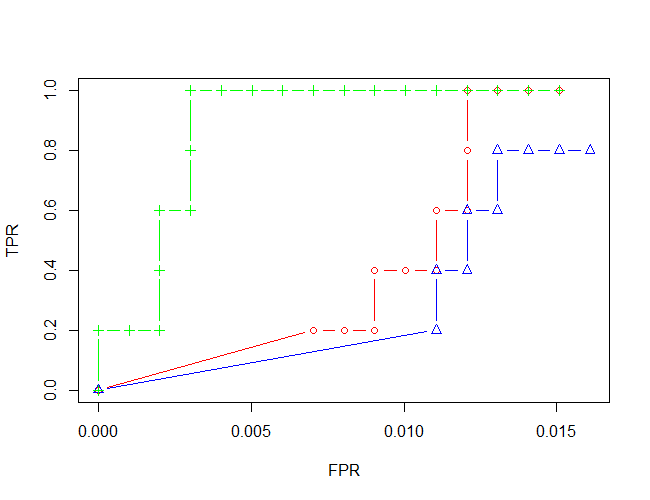
\includegraphics[width=\textwidth]{../plots/200sample09}
        \caption{}
    \end{subfigure}
    \begin{subfigure}[b]{0.3\textwidth}
        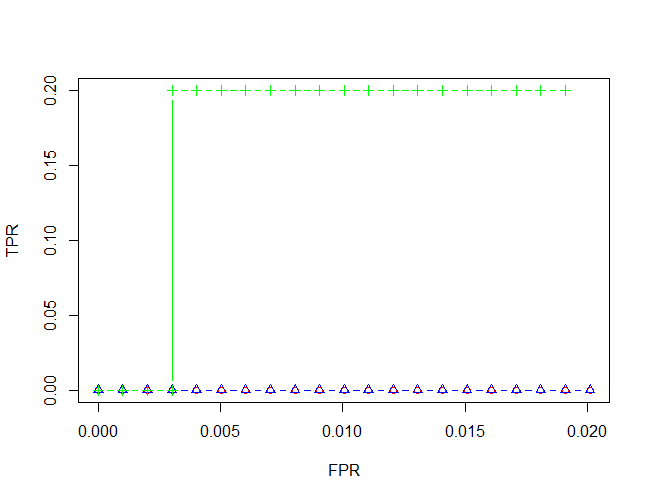
\includegraphics[width=\textwidth]{../plots/200sample06}
        \caption{}
    \end{subfigure}
    \begin{subfigure}[b]{0.3\textwidth}
        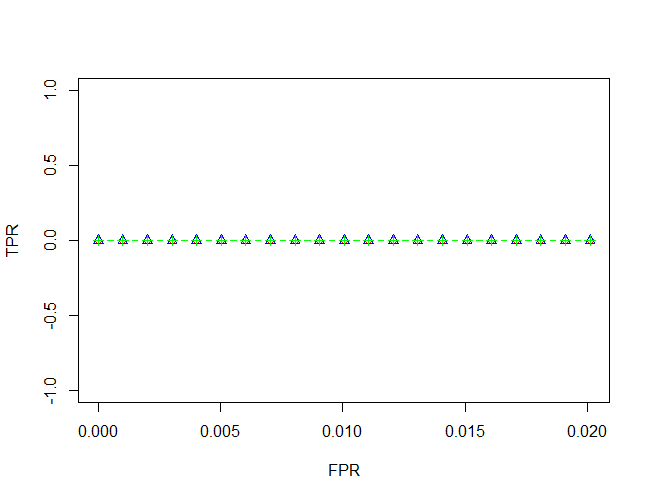
\includegraphics[width=\textwidth]{../plots/200sampe03}
        \caption{}
    \end{subfigure}
    \caption{ROC curves for three variants of the TCS algorithm in a VAR setting. Along each column $R^2 = \left \{ 0.9,0.6,0.3 \right \}$ ans long each row $n = \left \{ 500, 200, 100 \right \}$}.
    \label{general ROC plots}
\end{figure}

ROC curves for the above simulation are presented in Figure \ref{general ROC plots}. When the sample size is large all three methods are robust to the noise level. With $n = 500$ efficient tilting outperforms the other the other two methods, however its screening performance deteriorates as the sample size falls. This is likely because parameter estimates for the AR process used to used to estimate the error auto-covariance matrix become unstable in smaller samples. Stable tilting is overall robust to both the sample size and the noise level. For example in plot (f), where $n=200$ and $R^2=0.6$, stable tilting finds 80 percent of relevant predictors whereas the remaining method find only 60 percent. It should be noted that for moderate sample sizes and $R^2 \geq 0.6$ stable tilting does not perform much better than the original procedure. Given the high computational cost of stable tilting this suggests that in most settings regular tilting is sufficient. Unsurprisingly, with $n = 100$ and $R^2 = 0.3$ all three methods break down completely. 

\subsection{Robustness to additional assumptions}\label{robustness tests}

As expressed in Section \ref{seperation} some assumptions used to extend tilted correlations to the time series setting are quite restrictive. This section explores the effect of relaxing two assumptions which in real datasets may not be satisfied. To isolate the effect of relaxing the assumptions the sample size was varied over $n = \left \{ 500, 200 \right \}$ only, as Figure \ref{general ROC plots} shows that as all three methods performed well in this range. 

\subsubsection{Relaxing assumption A\ref{A8}}

Assumption A\ref{A8} requires that each predictor be independent of the error term $e_t$. To test the effect of relaxing the assumption innovations in the AR(1) error process were modified as shown below. The value of $r$ was again varied to attain $R^2 = \left \{ 0.9,0.6,0.3 \right \}$. 

\begin{align*}
    & e_t = 0.6e_{t-1} + \iota_t \\ 
    & \iota_t = w_t \cdot \sum_{j \in \mathcal{S}}x_{tj} \hspace{0.5cm} \text{with}\hspace{0.5cm} w_t \sim_{i.i.d.} \mathcal{N}\left ( 0,r^2 \right )
\end{align*}

Simulation results are presented in Figure \ref{testing A8 fig}. With $n = 500$ all three methods seem to perform well, although strangely stable tilting performs worse than the other two methods in plot (c), in which $n=500$ and $R^2=0.3$. The performance of efficient tilting is sensitive to high noise levels when the sample size is low. This may be explained by the fact that in the presence of heteroskedasticity AIC selects a higher order AR model, leading to even more unstable parameter estimates. 

\begin{figure}[h]
    \centering
    \begin{subfigure}[b]{0.3\textwidth}
        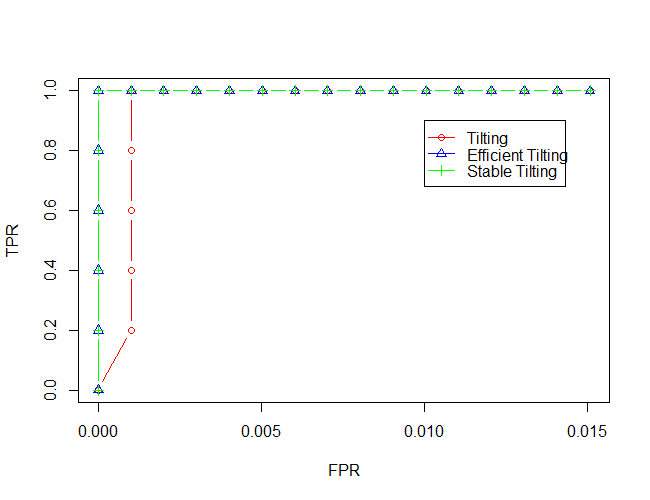
\includegraphics[width=\textwidth]{../plots/AR09}
        \caption{}
    \end{subfigure}
    \begin{subfigure}[b]{0.3\textwidth}
        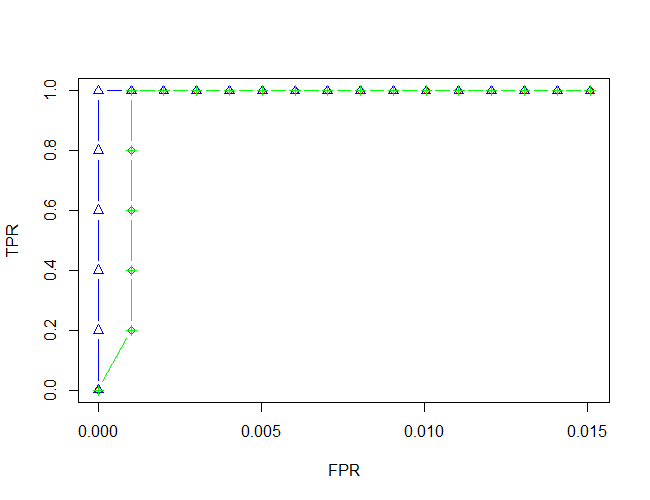
\includegraphics[width=\textwidth]{../plots/AR06}
        \caption{}
    \end{subfigure}
    \begin{subfigure}[b]{0.3\textwidth}
        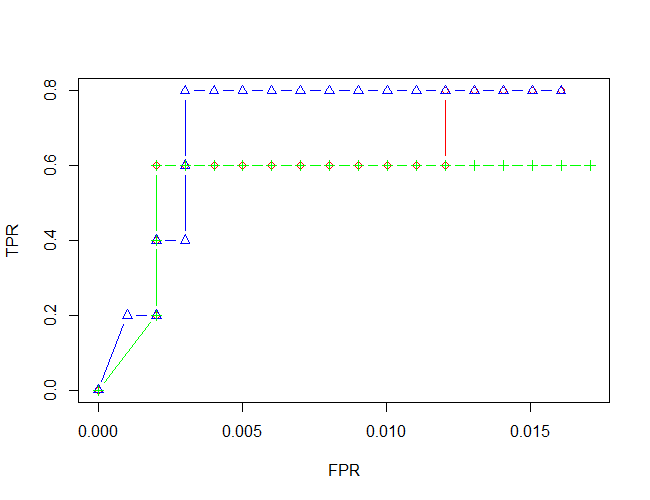
\includegraphics[width=\textwidth]{../plots/AR03}
        \caption{}
    \end{subfigure}
    \begin{subfigure}[b]{0.3\textwidth}
        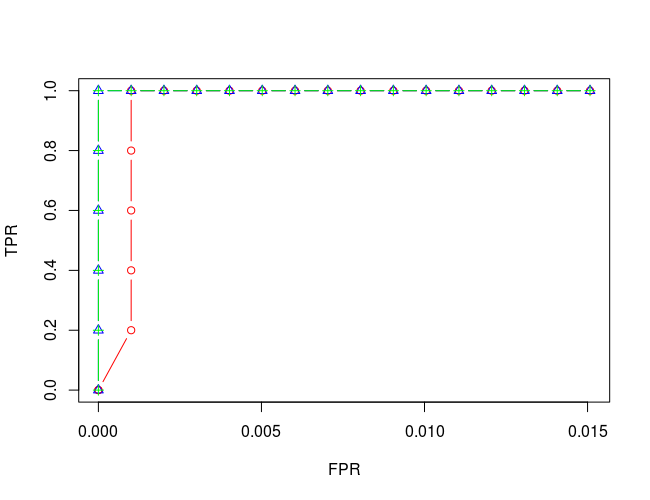
\includegraphics[width=\textwidth]{../plots/200AR09}
        \caption{}
    \end{subfigure}
    \begin{subfigure}[b]{0.3\textwidth}
        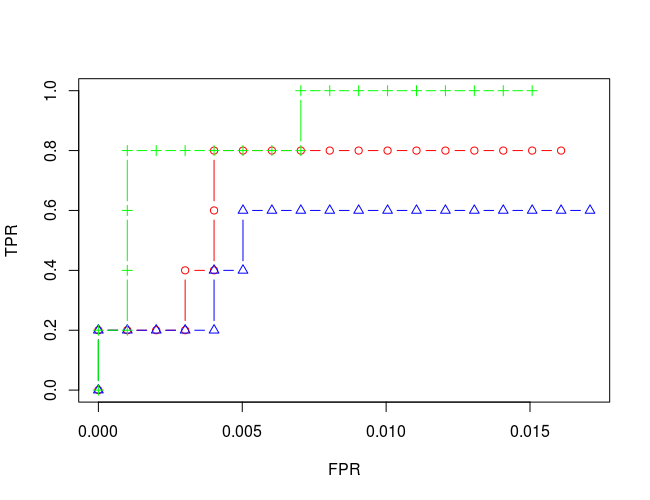
\includegraphics[width=\textwidth]{../plots/200AR06}
        \caption{}
    \end{subfigure}
    \begin{subfigure}[b]{0.3\textwidth}
        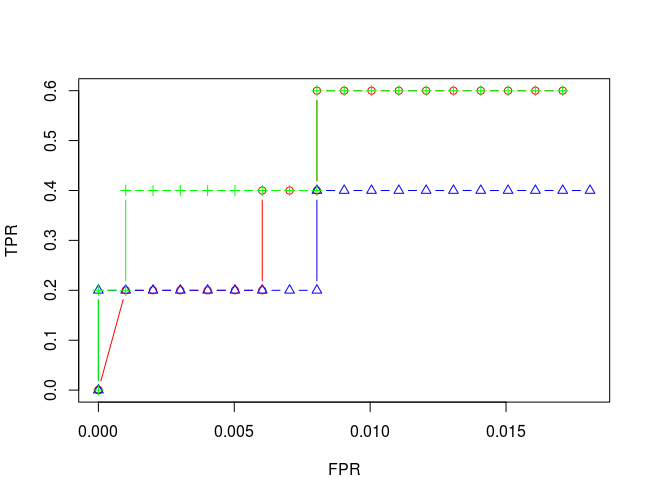
\includegraphics[width=\textwidth]{../plots/200AR03}
        \caption{}
    \end{subfigure}
    \caption{ROC curves for three variants of the TCS algorithm in a VAR setting with heteroskedasticity. Along each column $R^2 = \left \{ 0.9,0.6,0.3 \right \}$ ans long each row $n = \left \{ 500, 200 \right \}$}
    \label{testing A8 fig}
\end{figure}

\subsubsection{Relaxing assumption A\ref{A9}}

Assumption A\ref{A9} requires either that the predictors be bounded or that all of their moments exist. To test the  effect  of  relaxing  the  assumption innovations in the VAR(1) process were genertaed according to $\boldsymbol{\nu}_t \sim_{i.i.d.} \boldsymbol{t}_3\left ( \boldsymbol{0},\Sigma \right )$, where $\boldsymbol{t}_3$ represents a multivariate t-distribution with 3 degrees of freedom. The predictors are therefore unbounded and only the first two moments are finite. Note however that this setting is sufficient to guarantee consistency of regression parameters estimated via OLS. The shape matrix $\Sigma$ was set to equal the variance-covaraince in the multivariate Normal case, and values for $r$ were recycled from Section \ref{general comparison}. 

Simulation results are presented in Figure \ref{testing A9 fig}. Results are largely similar to those in \ref{general comparison}, with the exception that efficient tilting performs slightly worse when $n=200$ and the noise level is high. The fact that TCS algorithm does not break down completely confirms that A\ref{A9} is a purely technical assumption which arises from the strong mixing condition. In fact, similar results to Theorems \ref{theorem 1} and \ref{theorem 2} could have been proven using a number of dependence measures for time series processes. For example, the functional dependence measure of \cite{wu2005nonlinear} used in \cite{yousuf2018variable} allows for unbounded errors and predictors and only requires that a finite number of moments exist. 

\begin{figure}[h]
    \centering
    \begin{subfigure}[b]{0.3\textwidth}
        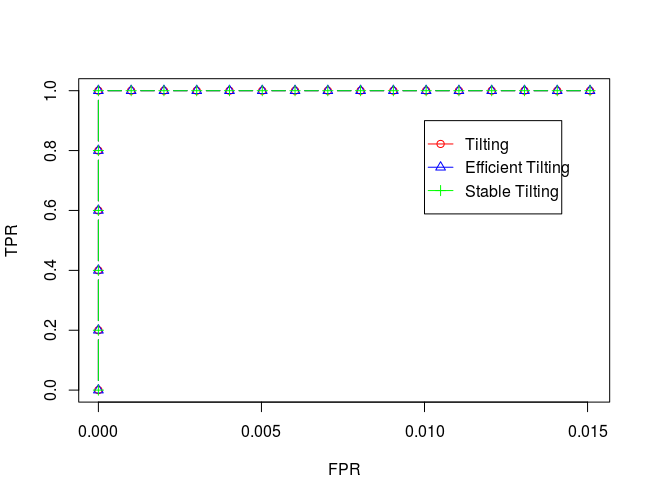
\includegraphics[width=\textwidth]{../plots/500t08}
        \caption{}
    \end{subfigure}
    \begin{subfigure}[b]{0.3\textwidth}
        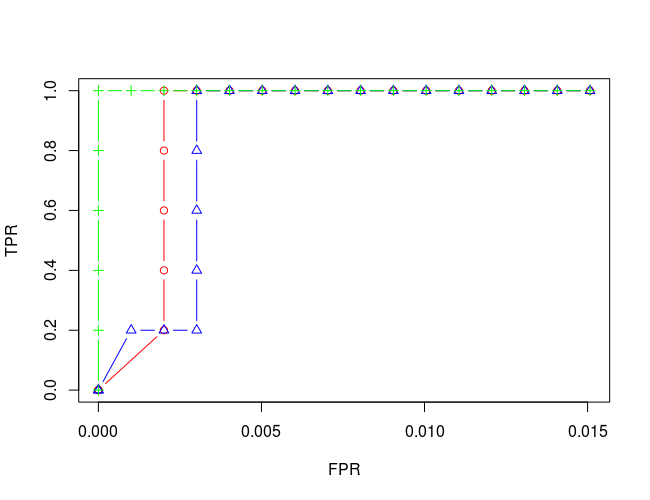
\includegraphics[width=\textwidth]{../plots/500t06}
        \caption{}
    \end{subfigure}
    \begin{subfigure}[b]{0.3\textwidth}
        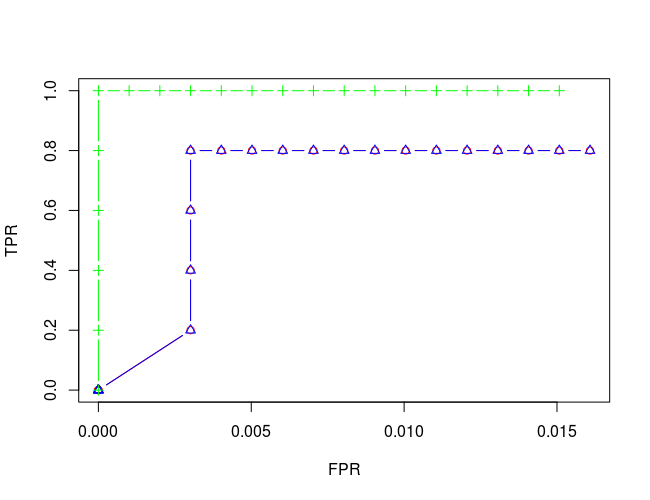
\includegraphics[width=\textwidth]{../plots/500t03}
        \caption{}
    \end{subfigure}
    \begin{subfigure}[b]{0.3\textwidth}
        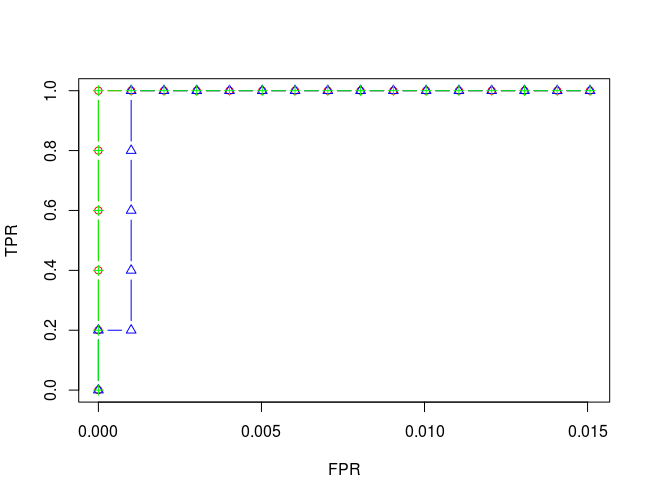
\includegraphics[width=\textwidth]{../plots/200t09}
        \caption{}
    \end{subfigure}
    \begin{subfigure}[b]{0.3\textwidth}
        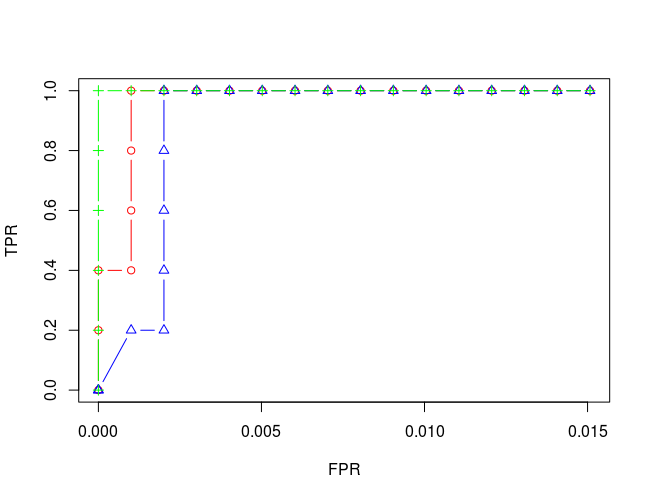
\includegraphics[width=\textwidth]{../plots/200t06}
        \caption{}
    \end{subfigure}
    \begin{subfigure}[b]{0.3\textwidth}
        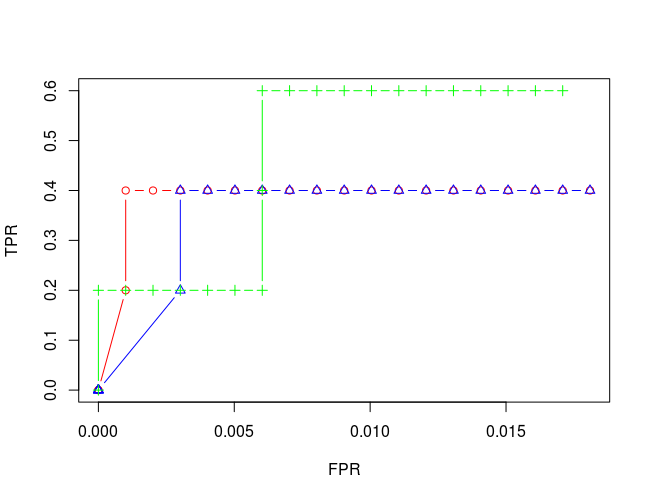
\includegraphics[width=\textwidth]{../plots/200t03}
        \caption{}
    \end{subfigure}
    \caption{ROC curves for three variants of the TCS algorithm in a VAR setting; only the first two moments of each predictor exist. Along each column $R^2 = \left \{ 0.9,0.6,0.3 \right \}$ ans long each row $n = \left \{ 500, 200 \right \}$}
    \label{testing A9 fig}
\end{figure}

\subsubsection{Disclaimer!}

Due to the high computational cost of stable tilting each of the ROC plots presented above is the result of a single simulation. The accompanying discussion is therefore only indicative of the relative performance of the three methods. Note however that results presented can be reproduced exactly using the R code provided on \href{https://github.com/Shakeel95/ST499-Tilting-}{GitHub}. 

\section{Forecasting UK macroeconomic time series}

To illustrate the practical utility of tilted correlations in a time series setting here I present a numerical study in which tilted correlations are used to select a model with which to forecast three key macroeconomic variables for the UK economy: 

\begin{equation*}
    \boldsymbol{y}_{t+1} 
    =\begin{pmatrix}
    y_{t+1,1}\\ 
    y_{t+1,2}\\ 
    y_{t+1,3}
    \end{pmatrix}
    = 100 \times \begin{pmatrix}
    \log(D7BT_{t+1}/D7BT_{t})\\ 
    \log(ABMI_{t+1}/ABMI_{t})\\
    \log(XUQABK_{t+1}/XUQABK_{t}) 
    \end{pmatrix}
\end{equation*}

These are roughly equal to the one period ahead percentage changes in quarterly inflation (D7BT), aggregate output (ABMI), and Sterling effective exchange rate (XUQABK67).

\subsection{Forecasting Setup}

\subsubsection{Data}

Data for this study was obtained from the Office for National Statistics (ONS) and Bank of England (BoE) websites. A large set of low frequency time series were collected by following \textit{Appendix D} of \cite{kapetanios2008forecast}, which explains how to reproduce the dataset used by \cite{stock2002macroeconomic} with UK data. All time series were transformed to achieve stationarity according to \textit{Appendix D}, and a summary of the data along with transformations applied is provided in Table \ref{data description}.

Since the Bank of England began using monetary policy to target inflation in 1992, and was granted independence in 1997, we can expect pronounced structural breaks in D7BT and XUQABK67 around this period. The data used therefore begins in the first quarter to 1998. The final set of predictors includes three factors obtained by taking principal components of the stationary predictors $\boldsymbol{x}_t$ and denoted by $\widehat{\boldsymbol{f}}_t = \left ( \widehat{f}_{t,1},\widehat{f}_{t,2},\widehat{f}_{t,3} \right )^T$. Additionally, the first three lags of $\boldsymbol{y}_{t}$ and $\boldsymbol{x}_t$ were added to the set for a total of $p = 110$ potential predictors.  

\subsubsection{Model selection with tilting}

The TCS algorithm set out in Algorithm \ref{tilting algorithm} was first used to reduce the number of potential predictors to an active set $\mathcal{A}$ of size $\left | \mathcal{A} \right | = m $. I followed \textit{Section 3.1} in \cite{cho2012high} in setting $m = \text{floor}\left \{ n/2 \right \}$. This value is designed to guarantee that projections performed by the algorithm are numerically stable while allowing a sufficiently large number of predictors to enter into $\mathcal{A}$. Where projections were numerically unstable the poorly conditioned matrix was augmented by adding a small amount of noise distributed according to $\mathcal{N}(0,0.001)$ to each entry prior to inversion.

Algorithm \ref{tilting algorithm} was run with tilted correlations from the original paper (Tilt), efficient tilted correlations introduced in Section \ref{efficient tilting} ($\text{Tilt}^E$), and stable tilted correlations introduced in Section \ref{stable tilting} ($\text{Tilt}^S$). A final model was obtained by applying the Lasso (+Lasso) to predictors in the active set $\mathcal{A}$, where the shrinkage parameter was selected via 10 fold cross-validation.

\subsubsection{Benchmark models}

The predictive performance of the TCS algorithm was bench-marked against forecasts from the four models presented in Table \ref{benchmark models}. These are models which are known to do well in practice, and consist of: a univariate auto-regression (AR), a vector auto-regression (VAR), and two factor augmented models (+F). Recently, forecasts from factor augmented models have garnered much attention; \cite{boivin2005understanding} for example note that institutions including the Federal Reserve of Chicago, the U.S. Treasury, the European Central Bank, the European Commission, and the Centre for Economic Policy Research are all investigating the performance of factor augmented models. Such models are considered useful as they offer a means of incorporating information from a large number of related time series while avoiding the curse of dimensionality. 

\begin{table}[h]
    \centering
    \bgroup
    \def\arraystretch{1.5}
    \begin{tabular}{c|c|c|c}
    \cmidrule(r){1-4}
    Model & Forecast & Parameter selection & Estimation \\
    \hline
    AR & $\widehat{y}_{t+1,j} = \widehat{c} + \sum_{\tau=1}^{p} \widehat{\phi}_\tau y_{t+1-\tau,j}$ & AIC & Yule-Walker \\
    VAR & $\widehat{\boldsymbol{y}}_{t+1} = \widehat{\boldsymbol{c}} + \sum_{\tau = 1}^{p} \widehat{\Phi}_\tau \boldsymbol{y}_{t+1-\tau}$ & AIC & Least Squares \\
    AR+F & $\widehat{y}_{t+1,j} = \widehat{c} + \sum_{\tau=1}^{3} \widehat{\phi}_\tau y_{t+1-\tau,j} + \sum_{k=1}^{3} \widehat{\gamma}_k \widehat{f}_{t,k}$ & 3 lags + 3 factors & Least Squares \\
    VAR+F & $\widehat{\boldsymbol{y}}_{t+1} = \widehat{\boldsymbol{c}} + \sum_{\tau = 1}^{3} \widehat{\Phi}_\tau \boldsymbol{y}_{t+1-\tau} + \widehat{\Gamma}_\tau \widehat{\boldsymbol{f}}_{t+1-\tau}$ & 3 lags + 3 factors & Least Squares*
    \end{tabular}
    \egroup
    \caption{Summary of benchmark models used in numerical study. The symbol * indicates the model was estimated according to \textit{Section II.C} of \cite{bernanke2005measuring}.}
    \label{benchmark models}
\end{table}

\subsection{Forecasting results}

Tables \ref{CPI table}, \ref{GDP table}, and \ref{exchange table} present the mean square forecast error (MSE), mean absolute forecast error (MAE), and average number of covariates selected (Size) for each method across each time series. Forecasts were produced using a rolling window scheme with $n = 50$ observations, and a total of 32 forecasts were made.  

Excluding the inflation time series, for which AR-type models performed best, forecasts obtained via tilting outperformed all four benchmark models in terms of MSE and MAE. Among the tilting variants stable tilting consistently produced the most accurate forecasts, followed by efficient tilting. Efficient tilting consistently selected a more parsimonious model than regular tilting, hence its improved performance may be due to the fact that a model with fewer parameters enjoys a lower forecast variance. However, stable tilting occasionally selected a larger model than regular tilting. This point to the fact that by selecting predictors on the basis of inclusion frequencies stable tilting was indeed isolating predictors which contributed to the true causal relationship with the response. 

Forecasts from multivariate models were consistently poor. However, the robust performance of AR type models across all three time series is impressive given the simplicity and low computational costs of these models.  Finally I note that factor augmented AR models outperformed AR models in roughly half of all cases, which contradicts the results of the numerical study presented in \textit{Section 7} of \cite{yousuf2018variable}.

\newpage
\begin{landscape}

\begin{table}
    \centering
    \begin{tabular}{|c||c|c|c|c|c|c|c|}
    \cmidrule(r){1-8}
     & AR(p) & AR(3) + F(3) & Tilt + Lasso & $\text{Tilt}^{E}$ + Lasso & $\text{Tilt}^{S}$ + Lasso & VAR(p) & VAR(3)+F(3) \\
     \hline
     MSE & $\boldsymbol{1.32\mathrm{e}{-3}}$ & $1.81\mathrm{e}{-3}$ & $2.02\mathrm{e}{-3}$ & $1.92\mathrm{e}{-3}$ & $1.94\mathrm{e}{-3}$ & $7.34\mathrm{e}{-3}$ & $3.14\mathrm{e}{-3}$ \\
     MAE & $2.99\mathrm{e}{-1}$ & $\boldsymbol{2.08\mathrm{e}{-1}}$ & $3.51\mathrm{e}{-1}$ & $3.36\mathrm{e}{-1}$ & $3.36\mathrm{e}{-1}$ & $6.95\mathrm{e}{-1}$ & $4.48\mathrm{e}{-1}$ \\
     Size & $5.84$ & $6.00$ & $7.00$ & $5.97$ & $5.56$ & $\boldsymbol{2.99}$ & $9.00$\\
    \hline
    \end{tabular}
    \caption{Average prediction errors and average number of predictors used, for seven models used to predict the quarterly percentage change in UK inflation measured via the consumer price index (CPI); lowest values for MSE, MAE, and average model size are in bold.}
    \label{CPI table}
\end{table}

\begin{table}
    \centering
    \begin{tabular}{|c||c|c|c|c|c|c|c|}
    \cmidrule(r){1-8}
     & AR(p) & AR(3) + F(3) & Tilt + Lasso & $\text{Tilt}^{E}$ + Lasso & $\text{Tilt}^{S}$ + Lasso & VAR(p) & VAR(3)+F(3) \\
     \hline
     MSE & $1.89\mathrm{e}{-3}$ & $1.43\mathrm{e}{-3}$ & $1.13\mathrm{e}{-3}$ & $1.10\mathrm{e}{-3}$ & $\boldsymbol{9.07\mathrm{e}{-4}}$ & $9.61\mathrm{e}{-3}$ & $3.17\mathrm{e}{-3}$ \\
     MAE & $3.45\mathrm{e}{-1}$ & $2.99\mathrm{e}{-1}$ & $2.69\mathrm{e}{-1}$ & $2.66\mathrm{e}{-1}$ & $\boldsymbol{2.22\mathrm{e}{-1}}$ & $7.69\mathrm{e}{-1}$ & $4.33\mathrm{e}{-1}$ \\
     Size & $\boldsymbol{2.81}$ & $6.00$ & $4.28$ & $3.97$ & $4.44$ & $2.99$ & $9.00$\\
    \hline
    \end{tabular}
    \caption{Average prediction errors and average number of predictors used, for seven models used to predict the quarterly percentage change UK gross domestic product (ABMI); lowest values for MSE, MAE, and average model size are in bold.}
    \label{GDP table}
\end{table}

\begin{table}
    \centering
    \begin{tabular}{|c||c|c|c|c|c|c|c|}
    \cmidrule(r){1-8}
     & AR(p) & AR(3) + F(3) & Tilt + Lasso & $\text{Tilt}^{E}$ + Lasso & $\text{Tilt}^{S}$ + Lasso & VAR(p) & VAR(3)+F(3) \\
     \hline
     MSE & $6.36\mathrm{e}{-2}$ & $8.09\mathrm{e}{-2}$ & $6.59\mathrm{e}{-2}$ & $6.43\mathrm{e}{-2}$ & $\boldsymbol{6.14\mathrm{e}{-2}}$ & $1.87\mathrm{e}{-1}$ & $9.17\mathrm{e}{-2}$ \\
     MAE & $1.90\mathrm{e}{0}$ & $2.16\mathrm{e}{0}$ & $1.99\mathrm{e}{0}}& $1.95\mathrm{e}{0}$ & $\boldsymbol{1.93\mathrm{e}{0}}$ & $3.66\mathrm{e}{0}$ & $2.47\mathrm{e}{0}$ \\
     Size & $2.34$ & $6.00$ & $2.34$ & $2.16$ & $\boldsymbol{1.38}$ & $29.91$ & $9.00$\\
    \hline
    \end{tabular}
    \caption{Average prediction errors and average number of predictors used, for seven models used to predict the quarterly percentage change in the effective exchange rate for Sterling against a basket of representative currencies (XUQABK67); lowest values for MSE, MAE, and average model size are in bold.}
    \label{exchange table}
\end{table}
\end{landscape}

\begin{table}[h]
    \centering
    \begin{tabular}{c|c|c|c}
    \cmidrule(r){1-4}
    Identifier & Source & Description & Transformation\\
    \hline
    UTKZ & ONS & Services price index & $\Delta^2 \log$ \\
    UTKX & ONS & Non-durable goods price index & $\Delta^2 \log$ \\
    UTLB & ONS & Semi-durable goods price index & $\Delta^2 \log$ \\
    UTKT & ONS & Durable goods price index & $\Delta^2 \log$ \\
    ABJS & ONS & Household final consumption expenditure (index) & $\Delta^2 \log$ \\
    PLLU & ONS & Output of manufactured products & $\Delta^2 \log$\\
    IUQAAMIH & BoE & Average of 4 UK Banks' base rates & $-$\\
    Rate & BoE & Official Bank Rate history & $-$\\
    D7BT & ONS & Consumer price inflation, all items & $\Delta \log$ \\
    XUQAERG & BoE & Average Effective exchange rate, Euro & $$\Delta \log$$\\
    XUQAUSG & BoE & Average Effective exchange rate, US \$ & $$\Delta \log$$\\
    XUQABK67 & BoE & Average Effective exchange rate, Sterling & $$\Delta \log$$\\
    FBYH & ONS & Change in Inventories, Retail & $\Delta \log$ \\
    FAJM & ONS & Change in Inventories, Wholesale & $$\Delta \log$$ \\
    DLWX & ONS & Change in Inventories, Other Industries & $$\Delta \log$$ \\
    ABJR & ONS & Household final consumption expenditure (£m) & $\Delta \log$ \\
    UTID & ONS & Total consumption, Durable goods & $\Delta \log$ \\
    UTIT & ONS & Total consumption, Semi-durable goods & $\Delta \log$ \\
    UTIL & ONS & Total consumption, Non-durable goods & $\Delta \log$ \\
    UTIP & ONS & Total consumption, Services & $\Delta \log$\\
    TMMI & ONS & Purchase of vehicles & $\Delta \log$ \\
    MGRZ & ONS & Number of People in Employment & $\Delta \log$\\
    ABMI & ONS & Gross Domestic Product & $\Delta \log$\\
    NRJR & ONS & Real Households' disposable income & $\Delta \log$
    \end{tabular}
    \caption{Summary of low frequency macroeconomic data used in numerical study along with Office for National Statistics (ONS) / Bank of England (BoE) identifier and transformation applied to achieve stationarity. }
    \label{data description}
\end{table}

\chapter{Conclusion} \label{conclusion}

This dissertation has studied the largely unexplored problem of feature screening for high dimensional linear models in a time series setting. This was done by extending the TCS algorithm of \cite{cho2012high} to the time series setting while assuming strong mixing conditions. In Section \ref{efficient tilting} an efficient variant of the tilted correlation measure was proposed. In section \ref{stable tilting} a stable variant of the tilted correlation was proposed. This extension adapted the principle of stability selection introduced by \cite{meinshausen2010stability} to generate a stable conditioning set for each predictor. Finally, simulation studies and a real data example in Chapter \ref{numerical} confirmed that all three methods are good at distinguishing relevant predictors from irrelevant predictors in a high dimensional time series setting, with stable tilting generally outperforming the other two methods. 

It would have been interesting to compare the screening performance of the TCS algorithm to other techniques adapted to the time series setting, such as GLSS of \cite{yousuf2018variable} and KSIS of \cite{chen2018semiparametric}. However, code for these methods was not provided, and the emphasis of this dissertation was to develop a new screening procedure as opposed to comaring existing ones. Stable tilting was carried out using the stationary bootstrap of \cite{politis1994stationary}. It would certainly have have been useful to develop a data driven procedure for choosing the block length. For example, the block length could have been chosen to minimise the MSE of bootstrap replicates used to estimate the covariance between two predictors.  

There are several directions in which the results presented in this dissertation may be extended. Numerical studies in Chapter \ref{numerical} show that stable tilting generally outperforms the other methods considered. An advantage of stable tilting is that it is robust to small changes in the data, however the method's computational cost may be an prohibitively high price to pay. Further work could investigate the estimating tilted correlations using a partitioned median regression, which is robust to outliers and far less computationally expensive. Additionally, Chapter \ref{numerical} revealed that efficient tilting was particularly sensitive to low sample sizes. It was speculated that parameter estimates for the AR process used to construct a weighting became unstable in low sample sizes. Further work could explore the possibility of choosing the order of the AR process by placing greater weight on the sample size, thus preventing highly unstable parameter estimates from being used in the weighting matrix. 

% \bibliographystyle{ksfh_nat}
\bibliography{ref}



\end{document}
